\documentclass[header.tex]{subfiles}
\begin{document}
\title{\plaintitle}

\numberofauthors{1}
\author{
  Nur Al-huda Hamdan \hspace*{0.9cm} Simon Voelker \hspace*{0.9cm} Jan Borchers\\
  \\
    \affaddr{RWTH Aachen University}\\
    \affaddr{52074 Aachen, Germany}\\
    \email{\{hamdan, voelker, borchers\}@cs.rwth-aachen.de}
}


\CopyrightYear{2018} 
\setcopyright{acmlicensed} 
\conferenceinfo{CHI 2018,}{April 21--26, 2018, Montreal, QC, Canada}
\isbn{978-1-4503-5620-6/18/04}\acmPrice{$15.00}
\doi{https://doi.org/10.1145/3173574.3173656}



\teaser{
%\begin{figure}
\centering
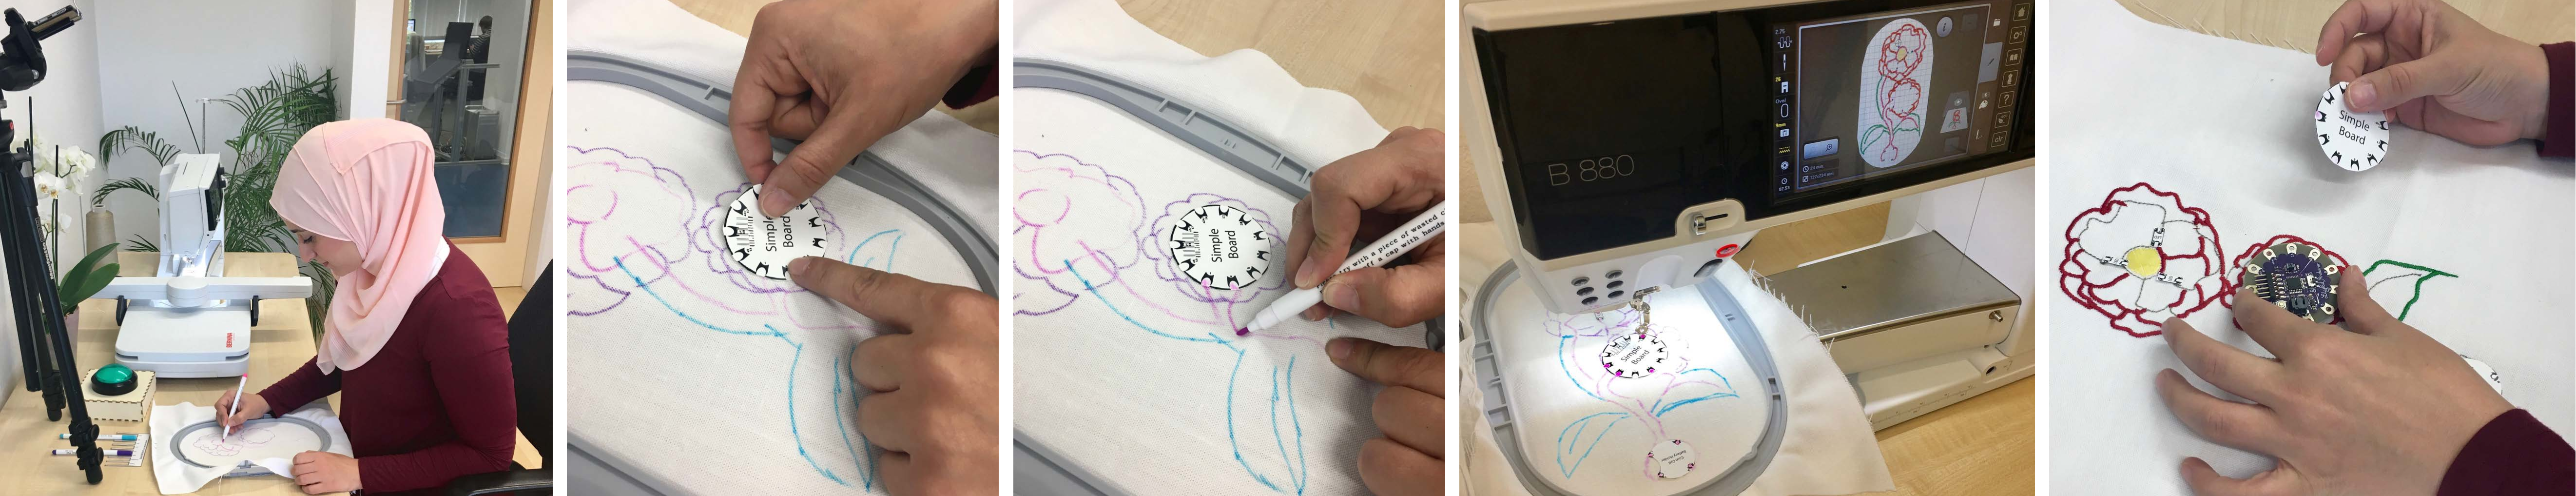
\includegraphics[width=1\textwidth]{figures/Fig1_Nur2}
\caption{Sketch\&Stitch workflow: 1. A user sketches artwork directly on fabric, 2. she uses \textit{Circuitry Stickers} to plan the circuit layout, 3. she draws circuit traces to connect the stickers, 4. the system takes a picture of the sketch, converts it into embroidery patterns, and sends them to an embroidery machine for stitching using conductive and non-conductive threads, 5. the user replaces Circuitry Stickers with real electrical components and attaches them to the fabric.
}
 \vspace{-1em}
\label{fig:Fig1}
}



\maketitle



\begin{abstract}
E-Textiles are fabrics that integrate electronic circuits and components. Makers use them to create interactive clothing, furniture, and toys. However, this requires significant manual labor and skills, and using technology-centric design tools. We introduce \textit{Sketch\&Stitch}, an interactive embroidery system to create e-textiles using a traditional crafting approach: Users draw their art and circuit directly on fabric using colored pens. The system takes a picture of the sketch, converts it to embroidery patterns, and sends them to an embroidery machine. Alternating between sketching and stitching, users build and test their design incrementally. Sketch\&Stitch features \textit{Circuitry Stickers} representing circuit boards, components, and custom stitch patterns for wire crossings to insulate, and various textile touch sensors such as pushbuttons, sliders, and 2D touchpads. Circuitry Stickers serve as placeholders during design. Using computer vision, they are recognized and replaced later in the appropriate embroidery phases. We close with technical considerations and application examples.
\end{abstract}



\category{H.5.2}{User Interfaces}{}

\keywords{\plainkeywords}

\section{Introduction}


Electronic textile technology enables people to create expressive, interactive, and functional textile artifacts for both playful and serious applications.
It combines the visual and haptic expressiveness of textiles with the interactivity and utility of electronic components such as LEDs, vibration motors, speakers, GPS receivers, and touch sensors. At the intersection of technology, art, and fashion (see, e.g., CuteCircuit.com), e-textiles have attracted artists, designers, hobbyists, and makers applying this technology in creative and artistic ways \cite{berzowska2005kukkia,Buechley:2010:LWH:1858171.1858206}. 
%Other e-fashion companies:
%https://iq.intel.com/fashion-metamorphosis-meet-the-butterfly-dress/
%http://ezratuba.com/wearable-tech
%Berlin University of the Arts - Department of Textile and Surface Design
This has motivated HCI research to investigate techniques that enable a wider audience to integrate fabrics and electronics into interactive textiles \cite{Buechley2009,perner2011handcrafting,5387040}.

In e-textiles, conductive threads, inks, polymers, or textiles are attached directly to a base fabric, creating \textit{fabric circuits}. These circuits connect traditional electronic components, usually on printed circuit boards, but they can also directly include functional parts such as fabric-based resistors, capacitors, touch sensors, actuators \cite{stylios2007shape}, or antennas \cite{catrysse2004towards}.
%batteries \cite{}
%powering elements \cite{}
Creating e-textiles typically involves 1.\ designing or choosing an artwork, 2.\ planning the layout of electrical components and traces, 3.\ creating the artwork and fabric circuit on the base fabric, 4.\ insulating circuit traces where necessary, and 5.\ attaching electronic components \cite{Lovell:2010:ETD:1810543.1810578}. 
The techniques for implementing e-textiles are based on traditional methods such as printing \cite{kim2010electrical}, weaving \cite{kallmayer2003new}, knitting \cite{farringdon1999wearable}, and  embroidery \cite{5387040}.
%\cite{castano2014smart,mattila2006intelligent}. These citations provide a review of methods

%Some of these techniques have been successfully adopted by the do-it-yourself community 
% as evident from makers' websites, such as Instructables\footnote{https://www.instructables.com/}, Sparkfun\footnote{https://www.sparkfun.com/} and Adafruit\footnote{https://www.adafruit.com/}. But these techniques have some constraints.
%More websites: https://www.lib.ncsu.edu/softcircuits


As users rely predominantly on manual fabrication of e-textiles \cite{Kazemitabaar:2017:MTA:3025453.3025887}, executing a design becomes labor-intensive and requires high skill levels as the number and density of electrical components and connections increase. Debugging e-textiles is only possible after investing considerable time in building them. Insulating circuit traces is an extra step requiring special tools and materials \cite{Buechley2009}. Observing participants in our e-textile workshops, and analyzing over 70 e-textile projects documented online, we found that this laborious multi-step process often forced them into trade-offs between the visual and functional aspects of their design, impeding improvisation and exploration. The lack of a design workflow and digital support for e-textile fabrication can thus limit the creative and iterative design of interactive textiles.
%enable users to focus and invest their time on the visual and functional aspects of their project.

% We analysed more than 70 e-textile projects on the mentioned websites and found that makers make a trade-off between the fidelity of the artistic pattern and the functionality of the artefact. 


In this paper, we present \textit{Sketch\&Stitch,} an interactive embroidery system that enables users to create e-textiles by sketching on fabric (Fig.~\ref{fig:Fig1}). It uses a computerized embroidery machine as a digital fabrication tool to handle the two most laborious steps when creating e-textiles, stitching and insulation. Yet, it maintains the physical and direct interaction between the user and the work piece during the creative tasks, designing and planning the visual and functional patterns.  Sketch\&Stitch features \textit{Circuitry Stickers}, printed adhesives representing elements users can embed into their design, from circuit boards and components, to wire crossings to insulate, to various textile touch sensors. These stickers guide the user while drawing circuit traces to ensure reliable electrical connections, and are recognized using computer vision, automatically generating stitch patterns for wire crossings, insulations, and sensors.

% In Sketch\&Stitch, a user begins by sketching an artwork on the workpiece fabric using colored fabric markers. She plans the placement of components using Circuitry Stickers and draws connections. When she is ready to execute the design, the system takes a picture of the sketch, converts it into embroidery patterns, and sends them to an embroidery machine. 
% %The embroidery machine's embedded display allows the user to verify the patterns and make minor adjustments before stitching is started. 
% The user may repeat these steps to review and test parts of her art and circuitry incrementally. Some Circuitry Stickers, e.g., for touch sensors, are already replaced with stitches automatically by the system. After embroidery is complete, the user replaces the remaining Circuitry Stickers with their component counterparts, using one of three attachment techniques we describe.

In the remainder of this paper, after reviewing related work, we first briefly introduce the particular features of computerized embroidery machines that are relevant for this work. We present the Sketch\&Stitch system and workflow. We illustrate the extensions we added to Sketch\&Stitch beyond the basic system that enable a wider range of practical applications, and walk the reader through a concrete example. After an evaluation of technical stitches for fabric circuits, we describe the software implementation. Finally, we present several example artifacts created by an artist using our system, and close by discussing the current limitations of the system and opportunities for future research.

In summary, this paper makes the following contributions:
\begin{itemize}
    \item Sketch\&Stitch, a new approach and system prototype to create e-textiles by drawing directly on the fabric;
    \item Interaction techniques and  embroidery patterns that let users include circuit boards, components, insulation, wire crossings, and a variety of fabric sensors using Circuitry Stickers;
    \item Technical evaluations of stitches for embroidering fabric circuits with digital embroidery machines.
\end{itemize}


% Machine embroidery has bloomed entering homes, makerspaces and design studios of crafters, hobbyists and DIY.

% \url{http://www.strategyr.com/MarketResearch/Sewing_Machines_Market_Trends.asp}

% \url{http://robyns.world/2015/06/13/infographic-sewing-machine-day/}


\subfile{RelatedWork}

\section{Embroidery Machines In Personal Fabrication}
%Computerized embroidery machines became available to homes and small business in the 1980s. At prices between 500 and 15,000 US Dollars, they 
Computerized embroidery machines have become a tool frequently found in schools, maker spaces, and small businesses \cite{lipson2010factory}, and are part of the MIT recommended Fab Lab inventory, for example.  %\footnote{fab.cba.mit.edu/about/fab/inv.html}, 
They use a hoop system to hold the fabric taut under the needle and move it automatically along the $x$ and $y$ axes during stitching. %stitch embroidery patterns. 
A presser foot, a metallic attachment that surrounds the needle, holds the fabric flat to prevent it from rising and falling with the needle. A control panel and embedded display provide basic functionality to, e.g., start/stop the machine, control thread tension, change stitching speed, view embroidery patterns and make minor adjustments such as re-positioning, scaling, rotating, mirroring, and re-ordering. Home embroidery machines can stitch up to 1000 stitch/min.


%  \begin{figure}
% \centering
%   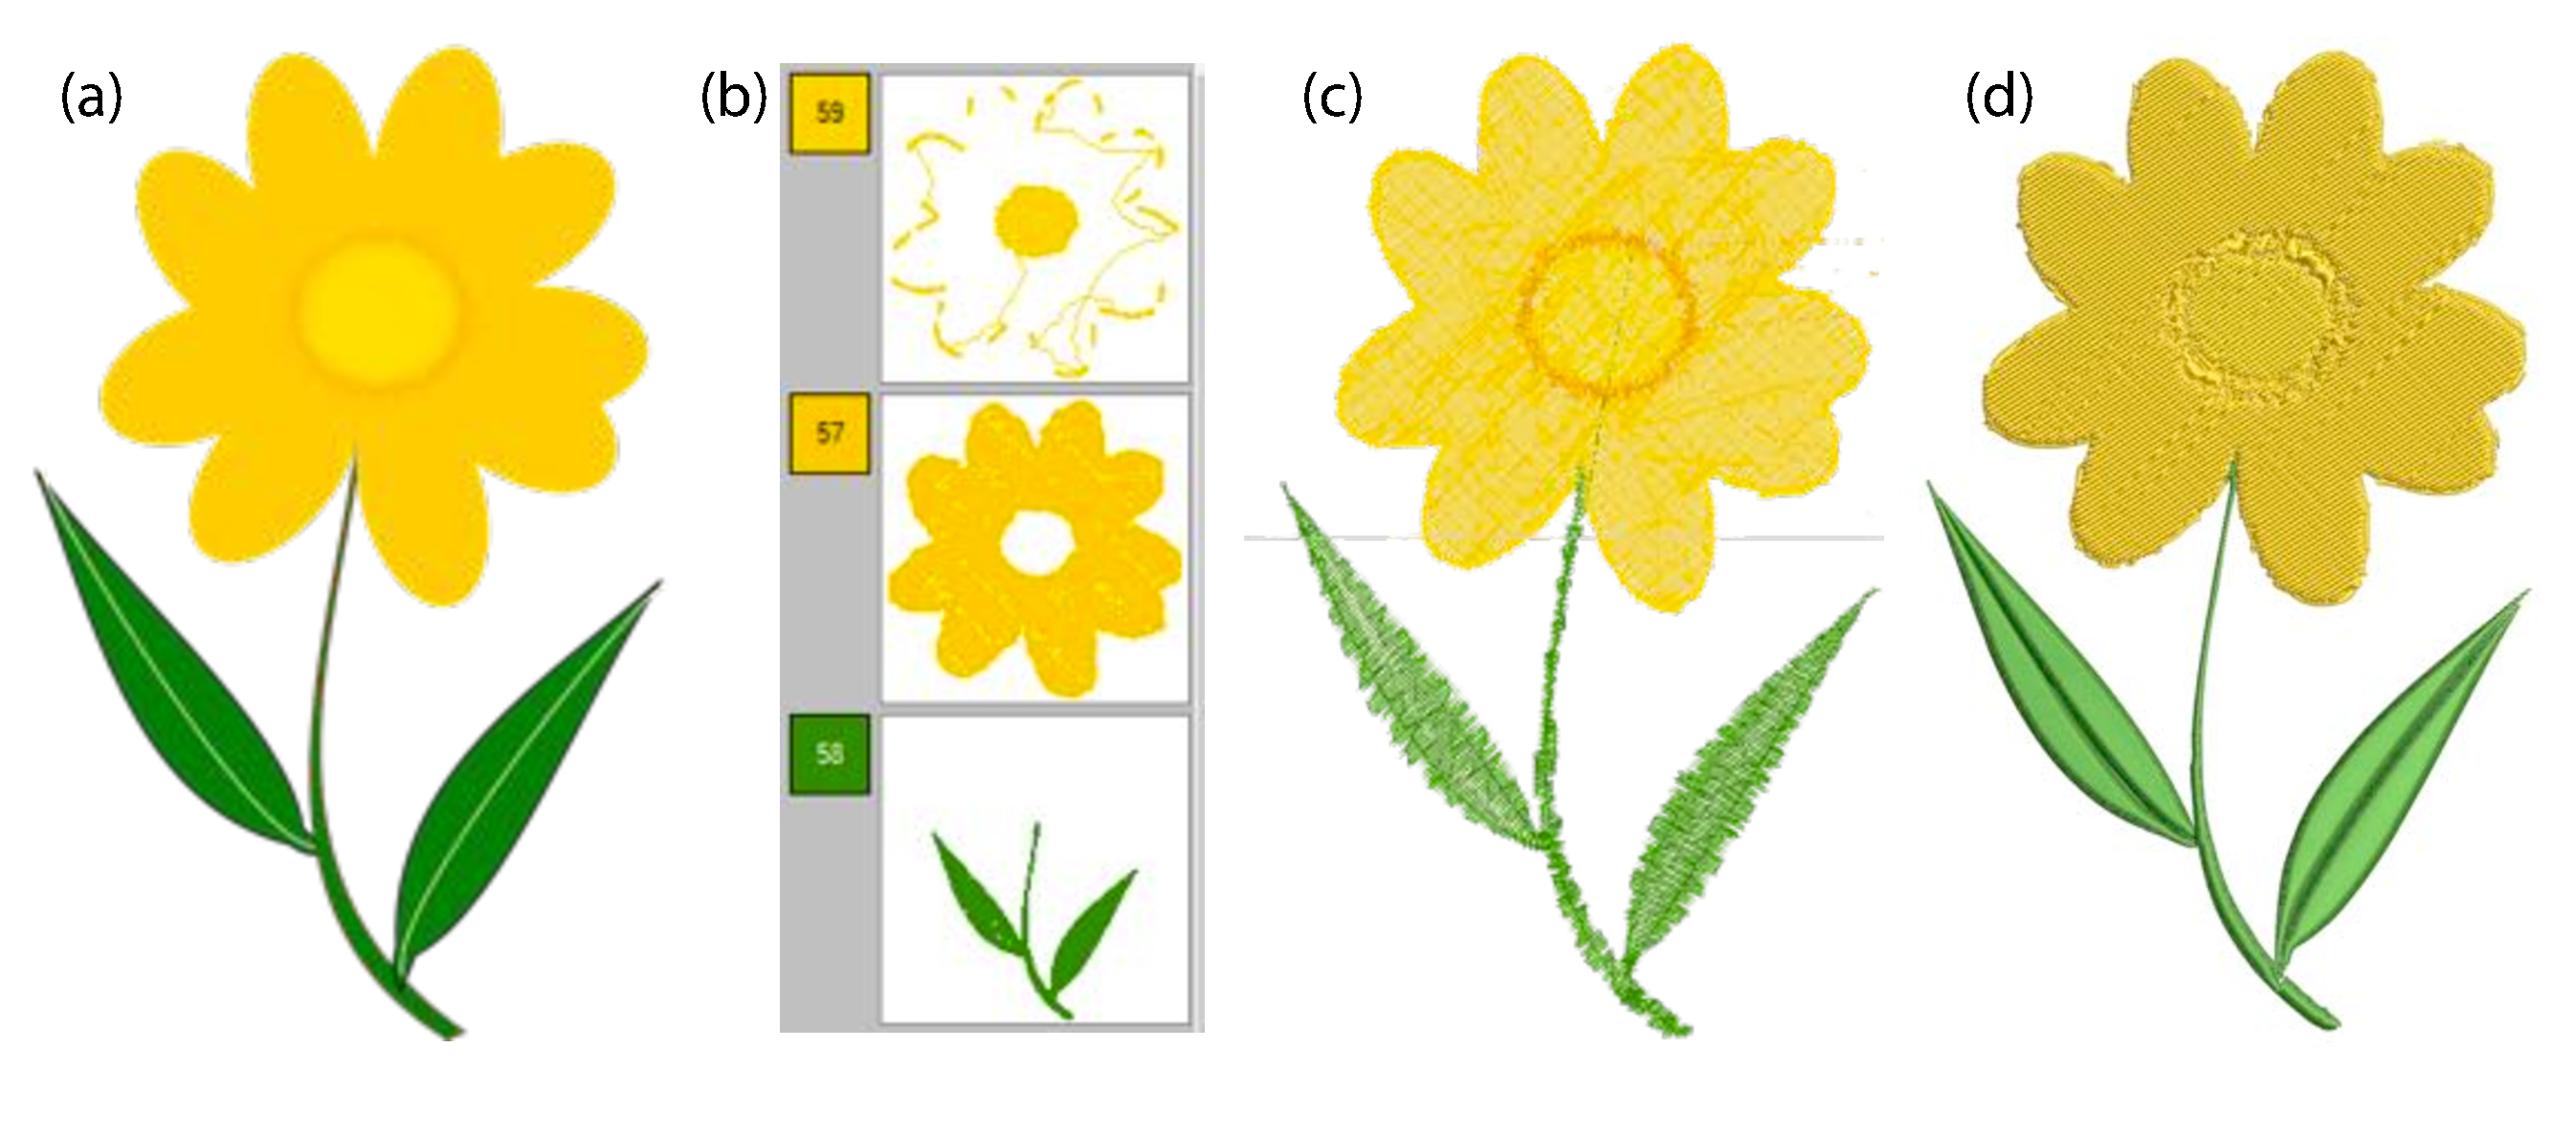
\includegraphics[width=0.9\columnwidth]{figures/EMWorkflow}
%   \caption{Image digitization in embroidery software: (a) imported image, (b) separation into color layers with assigned thread colors, (c) generated tool path, (d) final embroidery pattern }~\label{fig:EmbroideryWorkflow}
%   \vspace{-1.5em}
% \end{figure}

Embroidery machines come with proprietary software that runs on the user's computer. The software transforms color images into embroidery patterns and generates a tool path for the machine. The path dictates how an embroidery hoop moves under the needle. It includes stitch patterns, thread color changes, and jump stitches when traveling between different stitch objects. To optimize tool path generation, embroidery software separates design objects into multiple layers based on color. 
%(Fig.\ \ref{fig:EmbroideryWorkflow}). 
That way, the machine has to stop and prompt the user to manually change thread color less often. Jump stitches need to be trimmed automatically or manually. 
To reduce these jumps, professional embroidery designers often re-program patterns, manually sequencing stitch objects and individual stitches. 
%Industrial embroidery machines can change thread colors automatically. 
An embroidery machine reads a digitized embroidery pattern from a memory card or a computer connection, recognizes color layers, and stitches them sequentially.

%Virtual hoops help the user position, orient and scale a design relative to physical hoops. 
%Some software tools allow the user to print a design inside a virtual hoop in life-scale to assist the user in aligning the physical hoop on the workpiece fabric.

The internal algorithms that generate a concrete stitching pattern and tool path from a design encode advanced expertise in the mechanical properties of fabrics and threads, not unlike the slicing software turning 3D models into print head tool paths for 3D printers. This complexity is usually kept from the user, but embroidery software still has a relatively steep learning curve, offering a large number of visual design options and specialized tools for manipulating stitch patterns, such as a parametric stitch designer and pull compensation options.
Its user interface assumes a nontrivial amount of expertise in threads, fabrics, embroidery, and the workings of the machine.

\section{Sketch\&Stitch}
Sketch\&Stitch (S\&S) supports a new workflow for creating artistic e-textiles with embroidery machines. It lets users convert an idea sketched on fabric into an interactive system.  Users draw both artwork and electrical connections in free artistic shapes directly on fabric, without having to interact with CAD/CAM tools on a computer screen. S\&S captures the sketch and converts it into embroidery patterns. 
%Our workflow utilizes an embroidery machine to take over the laborious tasks in e-textile fabrication---stitching and insulating circuit traces. Yet, it maintains the physical and direct interaction between the user and the work piece during the creative tasks---designing and planning visual and functional patterns. 
%---> We miss the intelligence of layout software such as Fritzing or Autodesk's Eagle
%---> We miss the preciseness and manipulation of CAD tools
S\&S is designed with artists and makers in mind, enabling improvisational design and quick, low-threshold prototyping.
%The workflow with Sketch\&Stitch was developed with designers and makers in mind. 



The system comprises a smartphone on a mount above the work surface, a computer, a commercial embroidery machine, and a wireless button (Fig.\ \ref{fig:UI}). The smartphone runs our S\&S mobile app to capture a picture of the user's sketch and upload it to cloud storage. The computer runs our S\&S PC app and a proprietary embroidery software. %, DesignerPlus\textsuperscript{\textregistered} v.8. 
Our S\&S PC app digitizes the sketch, sends it to the embroidery software for conversion into embroidery patterns, and finally sends the patterns to the embroidery machine to be stitched. 


Users communicate with the system by sketching their art and circuit using colored pens and Circuitry Stickers on fabric.
%---> Why? Is this the best way of communication? Did we ask users?
To execute a design, the user places the fabric under the smartphone mount and presses the wireless button to capture a picture of her sketch. The S\&S PC app lets the user verify the digitized sketch and tune color detection using a simple slider-based user interface. The user sees the converted embroidery patterns on the embroidery machine's touch display. Optionally, the user may use the touch display to manipulate, e.g., scale, mirror, translate, or delete patterns. % ...also see the history of transformations
To start stitching, the user threads the machine's needle with the appropriate thread, and presses the start button on the machine.
% ...appropriate thread: conductive or non conductive (colored)
% Google Jacquard offers colored conductive threads for weaving. There is research of dying threads.

\textit{Circuitry Stickers} are symbolic images printed on adhesive paper. 
They are adhered to fabric to represent elements to be added to the circuit during and after embroidery. Sketch\&Stitch offers two types: \textit{Component Stickers} and \textit{Embroidery Stickers}. Component Stickers serve as placeholders for electronic components such as LEDs, motors and speakers, usually on PCBs. Users replace these stickers with their hardware counterparts after embroidery is complete, using one of three attachment techniques we describe further below. Embroidery Stickers represent multi-layer custom embroidery patterns required for wire crossings and our textile touch sensors. Users remove these stickers from fabric after capturing their design, and our system inserts the required patterns in place automatically during the embroidery process.

Circuitry Stickers were developed for two reasons: First, the presser foot in embroidery machines only has a clearance of about 1 mm above the fabric, too low to travel above even thin populated PCBs. For comparison, LilyPad PCBs are 0.8 mm thick but in total more than 2 mm high due to the SMD components. 
%This risks breaking the needle or machine if they come in contact.} 
Second, we wanted to save the user having to hand-draw the multi-layer patterns our textile sensors etc.\ require. Both kinds of stickers help users plan and sketch a circuit with ease and precision. Their adhesive backing allows experimenting with different layouts and holds them in place. % during design, and holds them in place while the fabric is being moved around.


The resulting end-to-end workflow is to 1.\ sketch an artwork directly on fabric with textile pens, 2.\ place Circuitry Stickers and draw connections between them, 3.\ capture the design via a camera, 4.\ remove any Embroidery Stickers and stitch the design on the embroidery machine, and finally 5.\ attach the electronics, replacing any Component Stickers. We look at these steps and our solutions for advanced features below.

%We aim to make e-textile creation accessible for emerging designers, hobbyists, crafters, and makers.
%To keep the traditional craft ways of entirely working on the physical workpiece, we developed a pipeline that enables users to sketch the design and plan the circuit directly on fabric. This pipeline 
% Simulating the traditional craft ways of directly interacting with the physical form using tools opens up a range of new creative possibilities [].
%Disconnect between physical and digital: There are numerous sources of variability in textile materials that can make a digital representation unstable, regardless of how good the simulation is.
% More agency and control over the final outcome [Being the Machine: Reconfiguring Agency and Control in Hybrid Fabrication].

\begin{figure}
\centering
  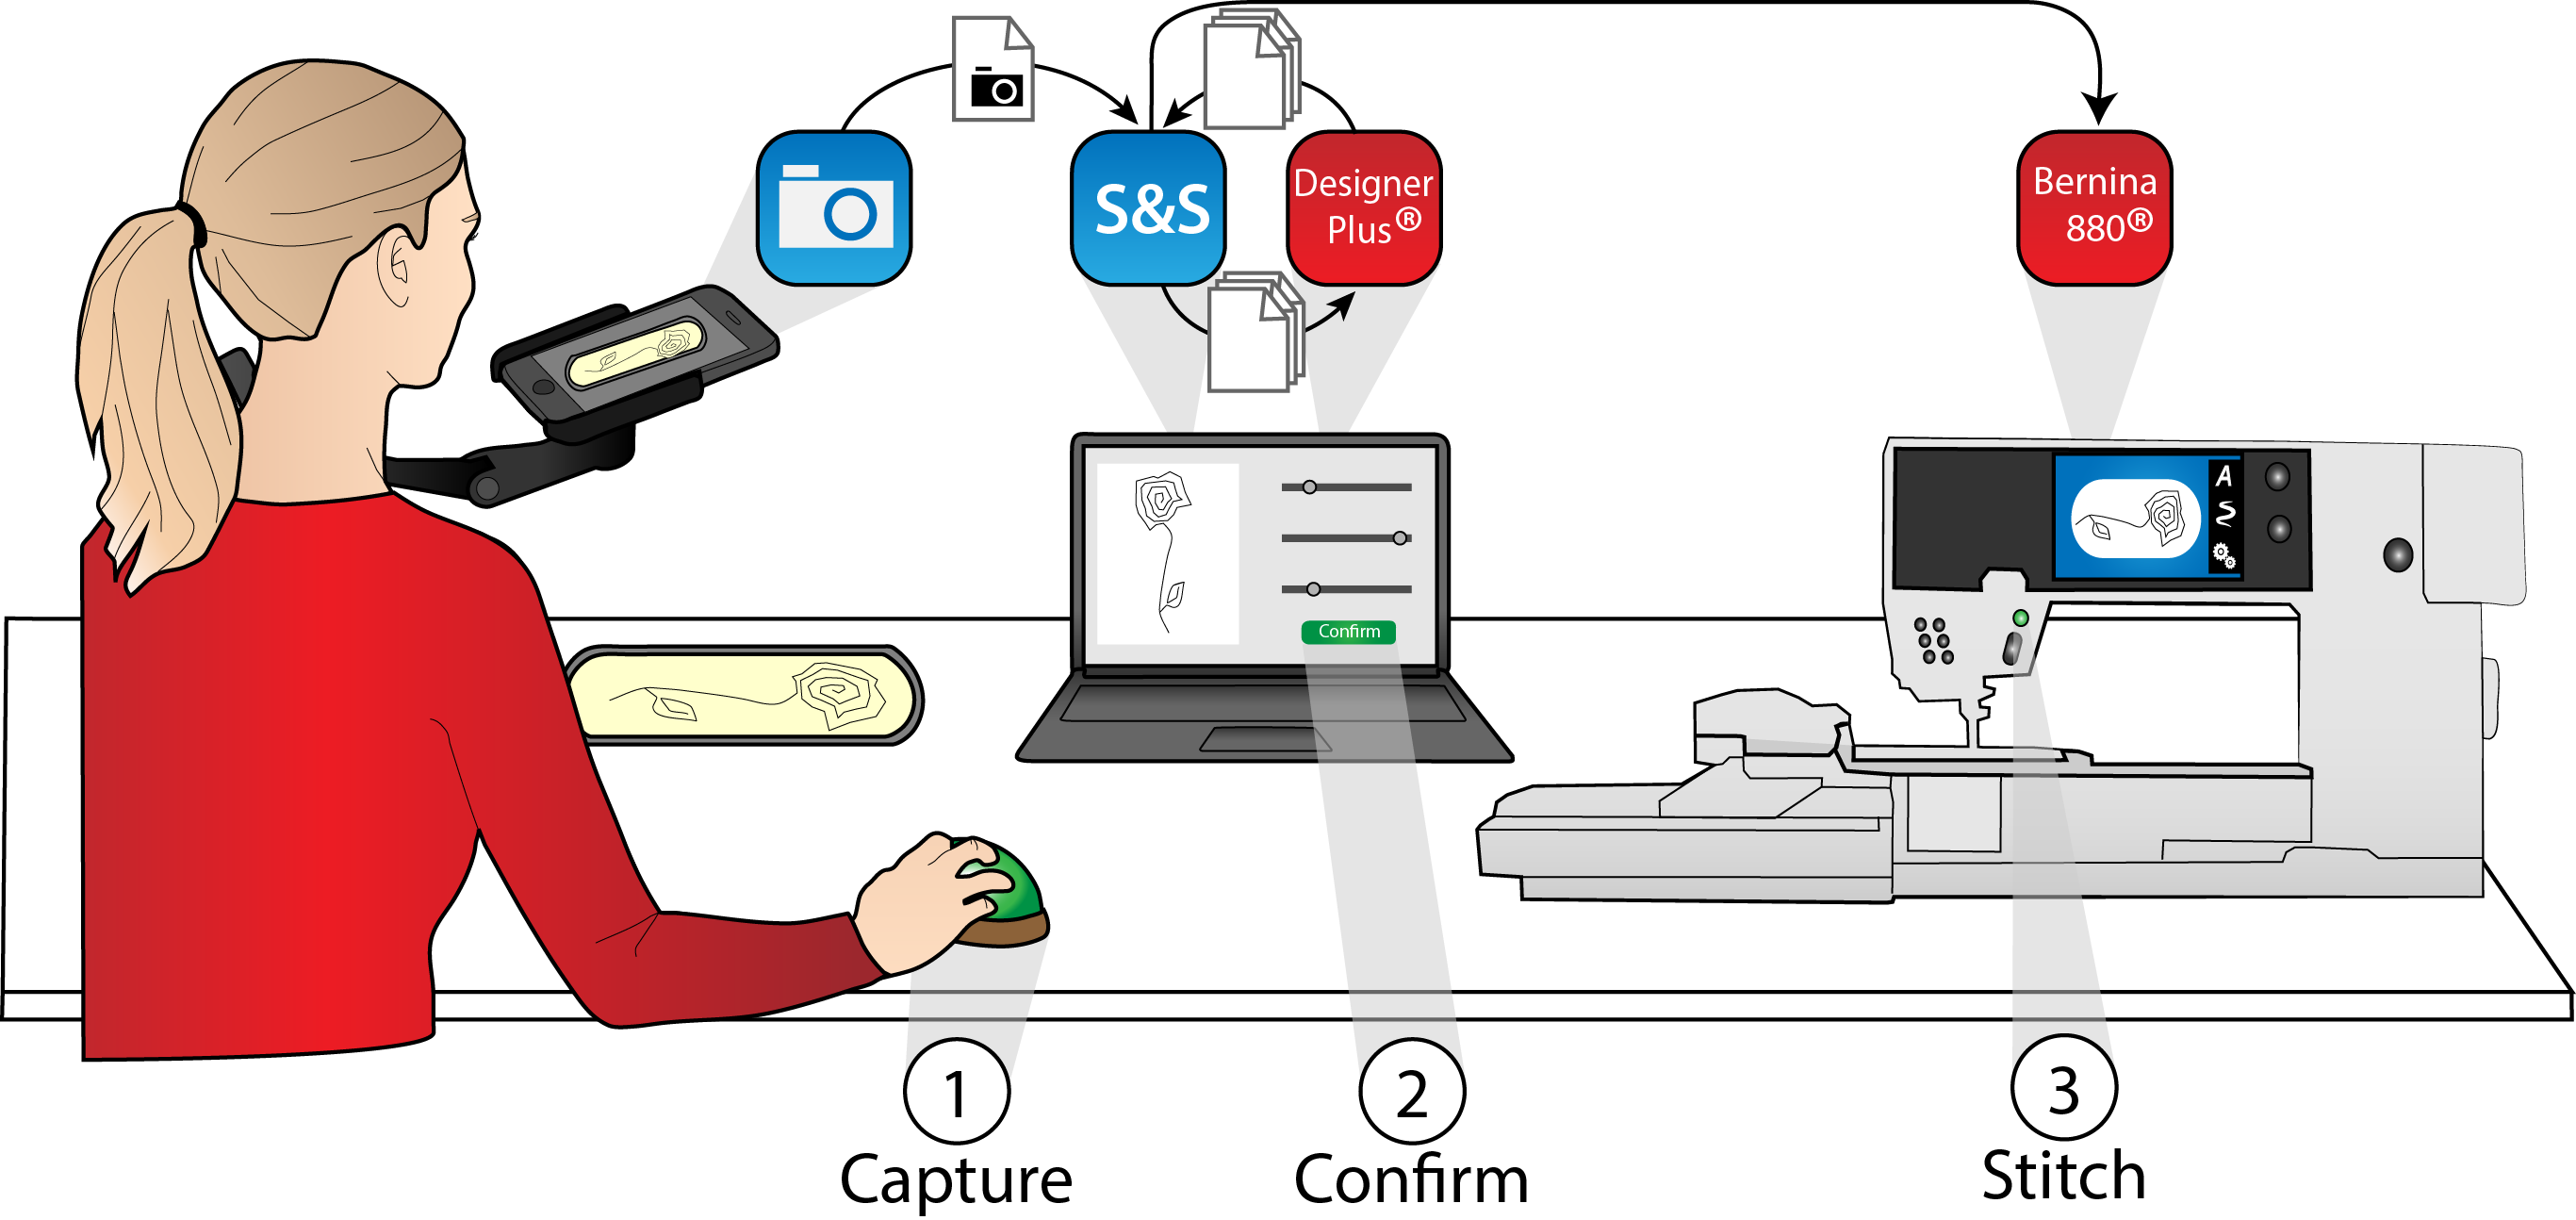
\includegraphics[width=1\columnwidth]{figures/UI.png}
  \caption{Sketch&Stitch comprise a smartphone, a wireless button, a PC, and an embroidery machine. It runs two custom softwares for capturing and digitizing sketches and a proprietary embroidery tool for converting images to stitches. Users capture a design with the button, verify it on the PC screen and stitch it in the embroidery machine.}~\label{fig:UI}
  \vspace{-2.2em}
\end{figure}


\subsection{Sketching on Fabric}

%Physical sketching provides users with continuous representation of their workpiece and helps them establish a closer relation with the materials (fabrics, threads, electronics) to better understand their properties and nuances \cite{willis2011interactive}. 

%Sketch\&Stitch allows users to draw their designs directly on fabric,
Physical sketching enables users to express themselves freely without the constraints of design applications \cite{landay1995interactive,Peiris:2014:PTC:2686612.2686691,schweikardt2000digital}, and provides a continuous representation of the evolving work piece \cite{willis2011interactive}. Drawing on fabric is an established art form. It is also used to design patterns for manual embroidery and mark the placement of pockets, buttons, and other design elements. 

At the beginning of the S\&S workflow, the user assigns her color palette---colors of the fabric pens that she will use in her sketch. Our system supports a palette of six colors: a \textit{trace color} for drawing electrical traces, an optional \textit{insulation color} for drawing insulated traces, and up to four \textit{art colors} for drawing the artwork. The system reserves the \textit{sticker colors} white and black for Circuitry Stickers. To assign the color palette, she uses our printable color template, which consists of six slits, each marked by a name: trace, insulation, or art, and an AR marker for optical detection. She places the template on the fabric and draws a stroke in each slit using water-soluble marking pens. The markings of these pens can be washed out easily when desired. She then captures the template by pressing a wireless button. The S\&S PC app provides feedback on the results of color assignment on the computer screen. After color assignment, the user secures the fabric flat and taut in an embroidery hoop of the desired size. The hoop has AR markers to localize the sketch. She now sketches her art and circuit.

Sketch\&Stitch uses colors instead of symbolic sketch annotations for user--system communication to avoid imposing design constraints on freehand sketches, and to keep the design uncluttered. Pen colors are used to encode stitch types and enforce the sequence of pattern stitching. For example, in a simple design, the system sequences all objects in \textit{trace color}, followed by objects in each \textit{art color}. This reduces the number of thread changes that the user has to do and enables her to debug her circuit before stitching the artwork. %(We describe stitch types in section Technical Stitching.) 
The number and color of threads for stitching the artwork can be chosen during the embroidery process, independently of the color palette. The user may pause the embroidery machine, re-thread the needle with a new thread, and resume stitching. % every time she wants to switch thread. % color. The machine resumes from the last stitch.}
%\textcolor{red}{(these are usually not the final \textit{thread colors}, see below).} 
 %The user repeats this process only if she wants to change the color palette.  
%\textcolor{red}{To be able to extend a partly stitched design in subsequent iterations, the user should avoid using thread colors from the color palette.}


The user can draw her art and circuit in any order.
To \textit{undo} any markings, she erases pen strokes by patting on the fabric with a damp cloth. She can undo stitched lines using a seam ripper. A design does not need to be complete to be stitched. At any point, the user can hit the button to take a photo, secure the hoop in the embroidery machine, and start the stitching process. This lets her evaluate and test her design early on, supporting \textit{incremental design}. For multiple iterations, the user should capture another photo of the embroidered fabric before making any new changes to avoid color confusion with stitched artwork (which can be of any thread color).

\subsection{Adding Electronics}
% The user places Component Stickers on the fabric to serve as placeholders for the electronics hardware to embed in the design. As illustrated above, embroidering with hardware components on the fabric is very challenging for most embroidery machines due to the low (\textasciitilde 1 mm) clearance of the presser foot. %For comparison, LilyPad PCBs are 0.8 mm thick but in total more than 2 mm high due to the SMD components.

Component Stickers have the same shape, size, and name as their physical counterparts. Fig.\ \ref{fig:ComponentStickers} shows a simple hand-sketched circuit that uses Component Stickers for the LilyPad kit. 
The grooves near the pin holes are added to guide the user and ensure that the connecting traces extend under the component and create sufficient contact surface for the attached board. 
%LilyPad components have exposed conductive plates on the top and bottom of the PCB.
The user prints Circuitry Stickers from the S\&S mobile app on adhesive paper using any printer. Stickers are tinted with \textit{sticker colors}. To use a sticker, she peels off its backing and adheres it to the fabric. %\textit{Embroidery Stickers} representing touch sensor areas can be cut to any desired size. 
Using the \textit{trace color} pen, she then draws circuit traces to connect the stickers. 
%The user may use a vinyl cutter to quickly cut them into shape. 
Component Stickers can be created for any PCB or off-the-shelf components. The only constraint is that they must have a pitch of at least 2.5 mm between their leads (see Technical Stitching). The stickers can be reused in later projects.


\begin{figure}[t]
\centering
  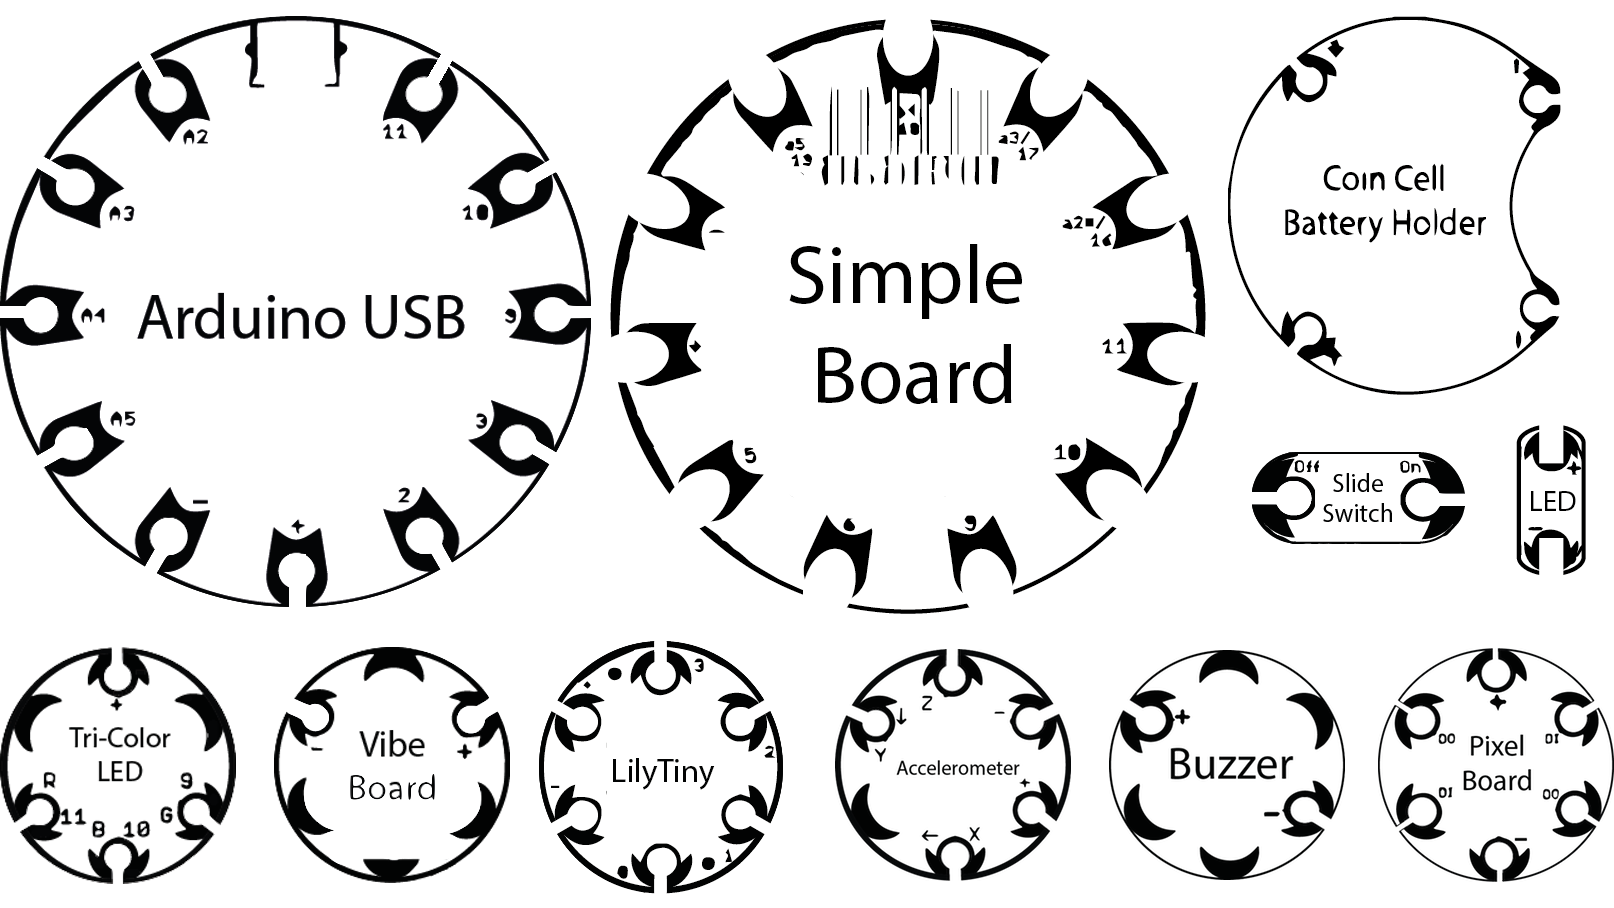
\includegraphics[width=0.85\columnwidth]{figures/ComponentStickers.png}
  \caption{1. Component Stickers represent electrical components in a hand-sketch circuit. Pin grooves designed to enlarge component contact area. 2. Stickers replaced with hardware cpunterparts after embroidery.}~\label{fig:ComponentStickers}
  \vspace{-2.2em}
\end{figure}

\subsection{Attaching Electronics}
%We mainly considered sewable components, and components with flat pads on the wrong side of the unit.

%Some stickers include grooves to guide users' traces to ensure reliable electrical connection with the added units. 


After embroidery is complete, the user replaces all Component Stickers with their corresponding hardware components and attaches them to the fabric.
%Sketch\&Stitch simplifies this step by stitching the contact surface  d. 
%Attaching hardware circuit boards and components to fabric is one of the main challenges in e-textiles. Researches have explored several techniques including soldering [], special soldering [], manual sewing [], breads [], ...
We describe three techniques for attaching electronics to fabric. The first uses 3M Electrically Conductive Tape 97033 (Z-tape), a double-sided adhesive that conducts in the $z$ dimension only when compressed. A piece of Z-tape is applied to the back of a component, the component is aligned to the stitched contact surface on the fabric and pressed down to create a connection. This technique is especially suitable for testing and prototyping a circuit, since it allows for easy removal, but can also be used for final attachment for e-textiles that are not handled much during use.

%We do not know if Z-tape can hold components with legs, we only tested with flat pads.



The second technique uses the embroidery machine. We developed the \textit{LilyStitch}, a custom stitch to attach components with 3 mm diameter pin holes. The stitch is a Single Running stitch in an M shape. This shape strengthens the attachment and forces the tie knots, which require more space than 3 mm, to be stitched outside the pin hole.  
%of the default line to to create a strong connection and
% with tie-in and tie-off knots on the wider end
%position of the fabric repeatedly, which can enlarge the hole and weaken the connection, and (b)
%Tie knots need space that 3mm is not encough for them
The length of the LilyStitch accounts for (a) the distance between the center of a pin hole and outer edge of the PCB (\textasciitilde 4 mm), and (b) the distance between needle point and the outer edge of the presser foot (\textasciitilde 5 mm). %Shorter distances lead to the presser foot pushing against the edge of the PCB when stitching close to it; longer distances weaken the stitch. 
Figure \ref{fig:LilyStitch} shows a custom embroidery pattern for attaching a board. LilyStitches were sequence-ordered manually to prevent the presser foot from traveling over the board during embroidery. This technique is very reliable and efficient for attaching sewable electronics. However, it requires accurate alignment between the physical component on fabric and the embroidery pattern. If an embroidery machine does not support such accuracy, users can stitch part of this pattern on fabric, align the component based on the stitches, then restart the embroidery. The physical component should be adhered to the fabric temporarily to keep it from moving. S\&S stores embroidery patterns for stitching LilyPad components on the embroidery machine. They can be accessed from the machine's touch display.

\begin{figure}[t]
\centering
  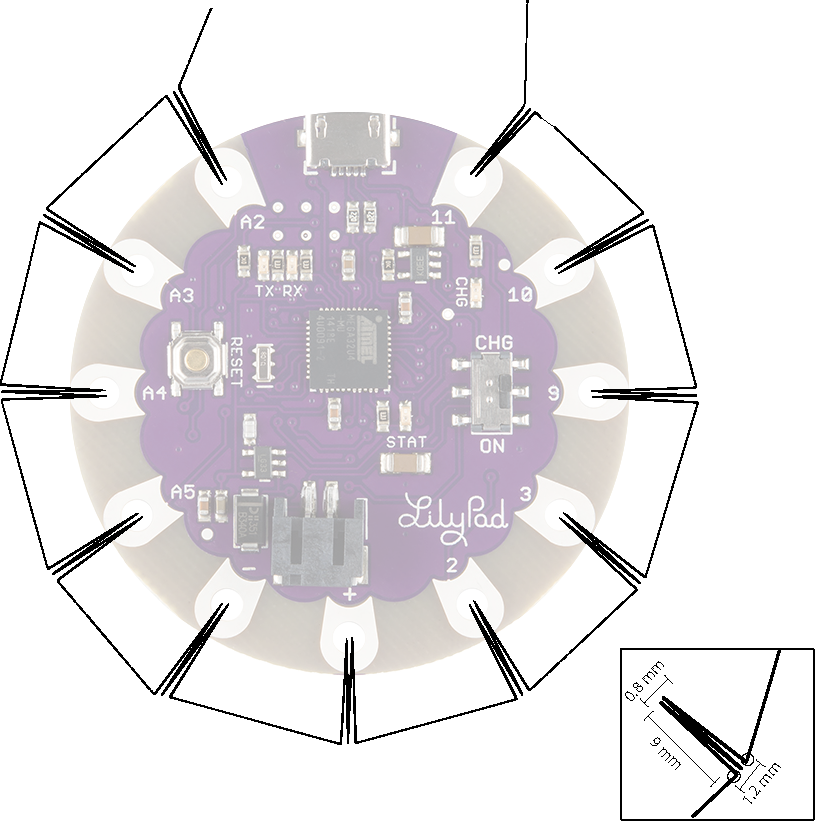
\includegraphics[width=1.0\columnwidth]{figures/LilyStitch}
  \caption{A custom embroidery pattern of LilyStitchs for attaching sewable electronics on fabric using an embroidery machine.}~\label{fig:LilyStitch}
  \vspace{-2.2em}
\end{figure}


%We recommend embroidering the hardware after the art and circuit patterns have been fully embroidered to avoid travel stitches.



The last technique uses the Button Sewing presser foot in sewing machines. The user has to manually align each pin hole under the presser foot. While this requires some skill, it becomes efficient with practice. Of course, the user can also manually sew into the holes using conductive thread as usual \cite{Buechley:2008:LAU:1357054.1357123}.
%And part stickers
The results of a sewing machine and manual sewing can be as reliable as using the embroidery machine, but they require more manual labor and time.


\subsection{Insulating Circuit Traces}
Insulating circuit traces, especially in wearable e-textiles, is paramount for their functionality. %Textiles are flexible materials. 
Exposed traces may come in contact with each other as fabric folds or bends, creating shorts or undesired signals. Buechley et al.\ \cite{Buechley2009} proposed couching---stitching one thread over another---as a natural insulation technique for fabric circuit traces. However, they noted that sewing machines may leave gaps in the couching stitch, making it an unreliable cover for the underlying conductive thread. Computer-controlled embroidery machines are much better at maintaining a consistent couching stitch, making them a perfect fit for this technique. 

The user insulates a trace in Sketch\&Stitch by drawing it using the \textit{insulation color} pen. The system detects objects in this color and creates an \textit{insulation stack}---a grid layer and an insulation layer. Each layer contains a copy of the objects and is converted to an embroidery pattern. The machine stitches the patterns in sequence using the corresponding stitch type. 


%the grid pattern is stitched first using a \textit{grid stitch} with conductive thread, and the insulation pattern is stitched next using an \textit{insulation stitch} with non-conductive thread.

While couching circuit traces has functional advantages, it has two pitfalls: It can have a pronounced visual impact on the design due to its thickness, and the build-up of stitches can reduce the flexibility of the base fabric. In textile touch sensors, couching can reduce the sensor's sensitivity.




 

%\textcolor{red}{The system duplicates all objects in \textit{insulation color}, and stores them in two design layers: the bottom layer, tinted with \textit{trace color}, and the top layer, tinted in \textit{insulation color}. The system uses trace and insulation colors to map stitch types (more in section Technical Considerations) layer colors are used to map to stitch types and to define the sequence of stitching layers in the embroidery software.}
%We describe this process further in Implementation section. 


\subsection{Handling Crossing Traces}
\begin{figure}[t]
\centering
  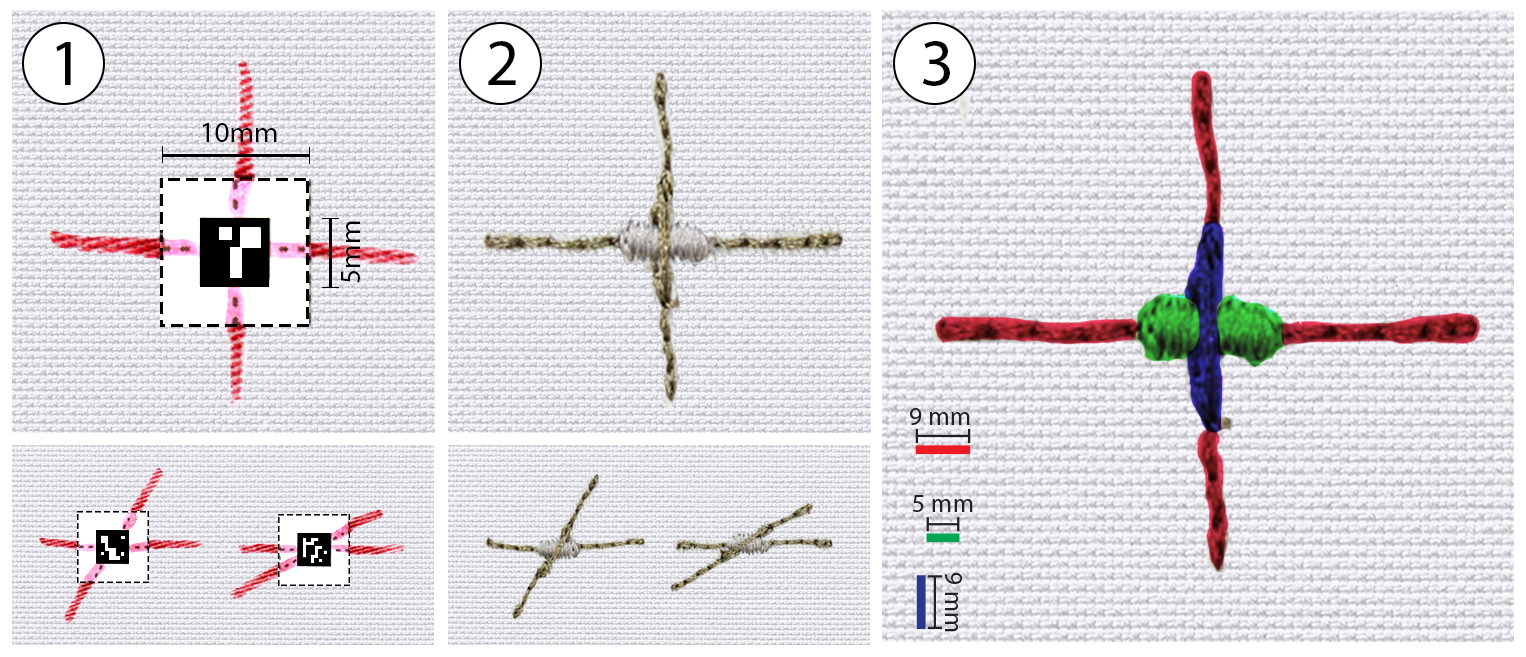
\includegraphics[width=1\columnwidth]{figures/ShieldStickers.png}
  \caption{1. Shield Stickers mark crossing traces (at 90\textdegree, 60\textdegree, 30\textdegree) on fabric. 2. Stitched shields. 3. Shield stack and pattern.}~\label{fig:ShieldStickers}
  \vspace{-2.2em}
\end{figure}

As the number of circuit elements increases in a design, the need for circuit traces crossing each other becomes inevitable. Dunne et al.\ \cite{Dunne:2012:MEC:2370216.2370348} manipulated the tension of the embroidery threads to allow two conductive threads to cross without touching. However, from our experience, this technique does not provide fail-safe insulation, especially when pressure is applied at the intersection point. Thread tension is determined by the fabric material, and changing it impairs the strength and appearance of stitches. It may also lead to ``thread birdnesting'', which causes the thread to tangle and the machine to stop.  
%various fabric-thread combinations require different tension settings and changing these settings may affect the appearance and strength of the stitches. 
S\&S provides users with \textit{Shield Stickers}, Embroidery Stickers to mark trace crossings to insulate on fabric.


To shield an intersection between two traces, the user places a sticker over the intersection point and draws connections between the traces on the sticker and her circuit traces using the \textit{trace color} pen (Fig.\ \ref{fig:ShieldStickers}.1). 
%Self crisscrosses of conductive thread are safe and do not need to be handled.
Embroidery Stickers have AR markers for optical detection. 
When the system detects the sticker, it creates a \textit{shield stack} in place. The stack is composed of a grid layer, an insulation layer, and a bridge layer. The grid layer contains a line segment to connect one of the user's traces. The insulation layer contains a line segment to couch the bottom segment. The bridge layer contains a line segment that bridges the user's second trace over the intersection. Objects in the \textit{bridge layer} are stitched using the \textit{bridge stitch} which connects two separate traces (up to 9 mm apart) without stitching between them. The layers are converted to embroidery patterns (Fig.\ \ref{fig:ShieldStickers}.) and stitched in sequence using the corresponding stitch type. 



\subsection{Adding Interactivity}
% \begin{figure}
% \centering
%   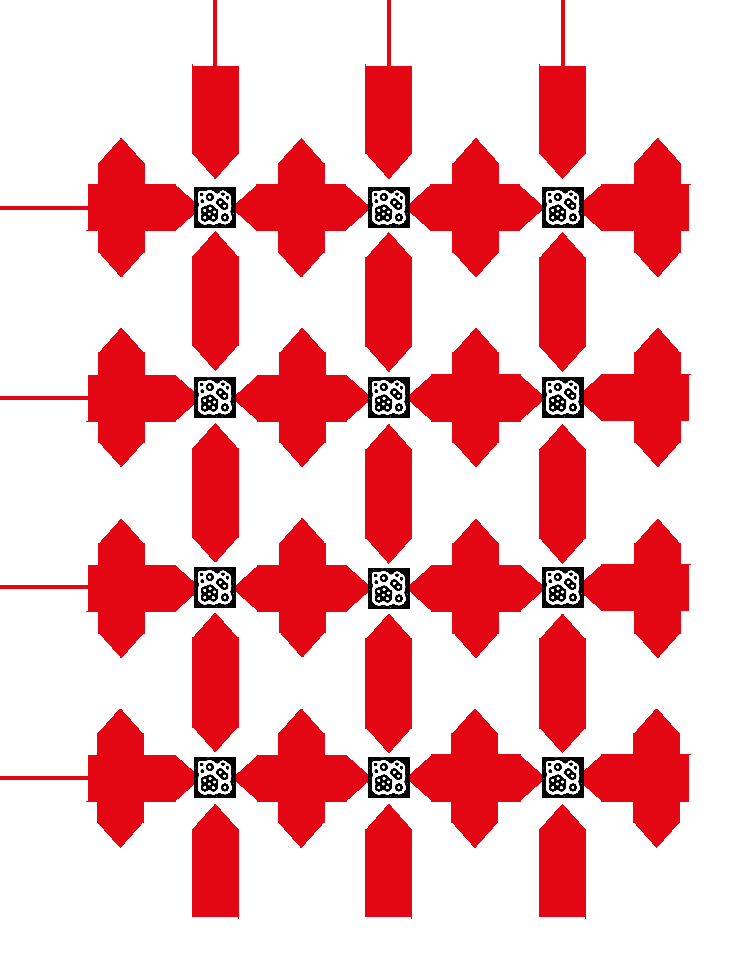
\includegraphics[width=0.6\columnwidth]{figures/RedStickers}
%   \caption{}~\label{fig:RedStickers}
%   \vspace{-2.5em}
% \end{figure}
Besides hardware electronics, users can use \textit{Sensor Stickers}, Embroidery Stickers to add touch sensors made from conductive thread directly onto the fabric. Sketch\&Stitch supports three sensor types: a pushbutton, a slider, and a touchpad.
%actuators, e.g., by couching a shape memory alloy wire, and various touch sensors, as we will demonstrate in this section.

Figure \ref{fig:PushButtons_Sliders} shows hand-sketched pushbuttons and sliders. A capacitive pushbutton is created by connecting any segment of conductive thread to a capacitive sensing circuit. The circuit can sense when the user's finger or body is in contact with the thread (touch) or not (no touch). A resistive pushbutton can be created with two conductive traces 3--4 mm apart that the user bridges when touching. %, with one trace usually grounded, the other connected to power or a controller pin. 
A slider can be implemented by placing several pushbuttons next to each other. %A resistive circuit enables a slider with coarse resolution---the user bridges two neighboring buttons. 
A capacitive circuit can interpolate the position of a finger on a slider based on the amount of surface area it covers, allowing  for high input resolution with limited wiring.  Using these simple techniques, users can create physical widgets of custom shapes and convert parts of their artwork to touch-enabled surfaces, by using the \textit{trace color} to draw those parts.

%When the user touches the two segments at the same time, a resistive sensing circuit registers a touch.

 % and its influence on neighbouring buttons.

% to determine more than one capacitive threshold for a single button. As the user's body comes in contact with more surface o with a capacitive sensor is interacted with by the user, the larger the capacitance will be. 



A matrix of pushbuttons, with each button connected to one IO pin, can be used as a 2D touchpad \cite{hamdan2016grabrics,5387040}. 
%offers the ability to detect all buttons being pressed at the same time, i.e., multi-touch. 
However, a 4$\times$4 touchpad would require 16 pins and traces. This complicates the wiring and may require additional hardware. Instead, using a layout of grid lines with time-multiplexing, as used in capacitive touchscreens, provides a sensor surface area capable of detecting individual touches, simple gestures, and sub-sensor point detection. It requires fewer pins 
%($4+4=8$ for a 4$\times$4 pad) 
and less power than scanning individual buttons. 
%However, it cannot support multi-touch. A grid layout can be connected to a capaciiuve or resistive circuit. But due to the low resistivity of the human finger, not all hardware can detect a direct touch. One alternative is to use pinching as an input technique. Hamdan et al. [] were able to detect the location and angle of a pinch on a matrix of resistive textile buttons using simple machine learning algorithms.
%Based on design recommendations from Texas Instruments for capacitive touch sensing with their MSP430 microcontroller\footnote{ www.ti.com/lit/an/slaa363a/slaa363a.pdf}, 
We applied the concept of a Shield Sticker to a grid layout and created the Sensor Sticker. The sticker enables 1D and 2D touch sensors to be automatically stitched on a single fabric layer. Figure \ref{fig:Touchpad} illustrates how users can add a touchpad sensor to fabric. The sticker can be cut in any convex shape and connected to a touch sensing Component Sticker via a \textit{trace color} pen. %: the user 1. cuts a Sensor Sticker in any convex shape, 2. adheres it to the fabric, and draws connecting traces from the sensor's grid lines using the \textit{trace color} pen, 3. captures the design and removes the sticker, finally, 4. 
The system replaces each grid point in the Sensor Sticker with a \textit{shield stack} and stitches the sensor. 




To evaluate our touchpad sensor, we overlaid two pieces of fabric over two 4$\times$4 sensors of 7 mm and 9 mm pitch. The fabrics were pre-marked with 9 touch locations each. We measured the error in distance between the touch location on the upper fabric and the measured location on the lower fabric (we used TI's MSP430G2553 MCU). We collected a total of 126 readings. The average error in both dimensions for the 7 mm sensors was ($M = 3.7 mm , SD = 1.5 mm$) and for the 9 mm sensor ($M = 2.2 mm, SD = 0.7 mm$).  Highest accuracy was achieved when the touch location was on top of a grid point. A 9 mm sensor can interpolate one touch point. Embroidering a 4$\times$4 sensor of 9 mm pitch requires less than 10 minutes.

\begin{figure}[t]
\centering
  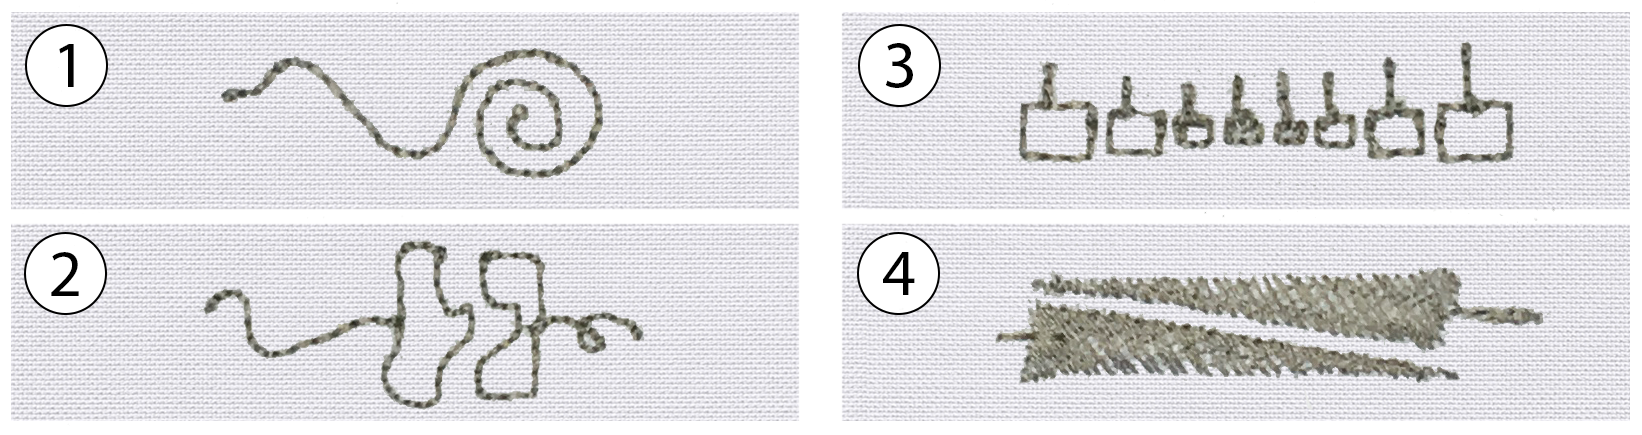
\includegraphics[width=1\columnwidth]{figures/PushButtons_Sliders.png}
  \caption{Hand-sketched sensors stitched with conductive thread. 1. Capacitive pushbutton. 2. Resistive pushbutton. 3. and 4. Sliders.}~\label{fig:PushButtons_Sliders}
  \vspace{-2.2em}
\end{figure}

\begin{figure}[h]
\centering
  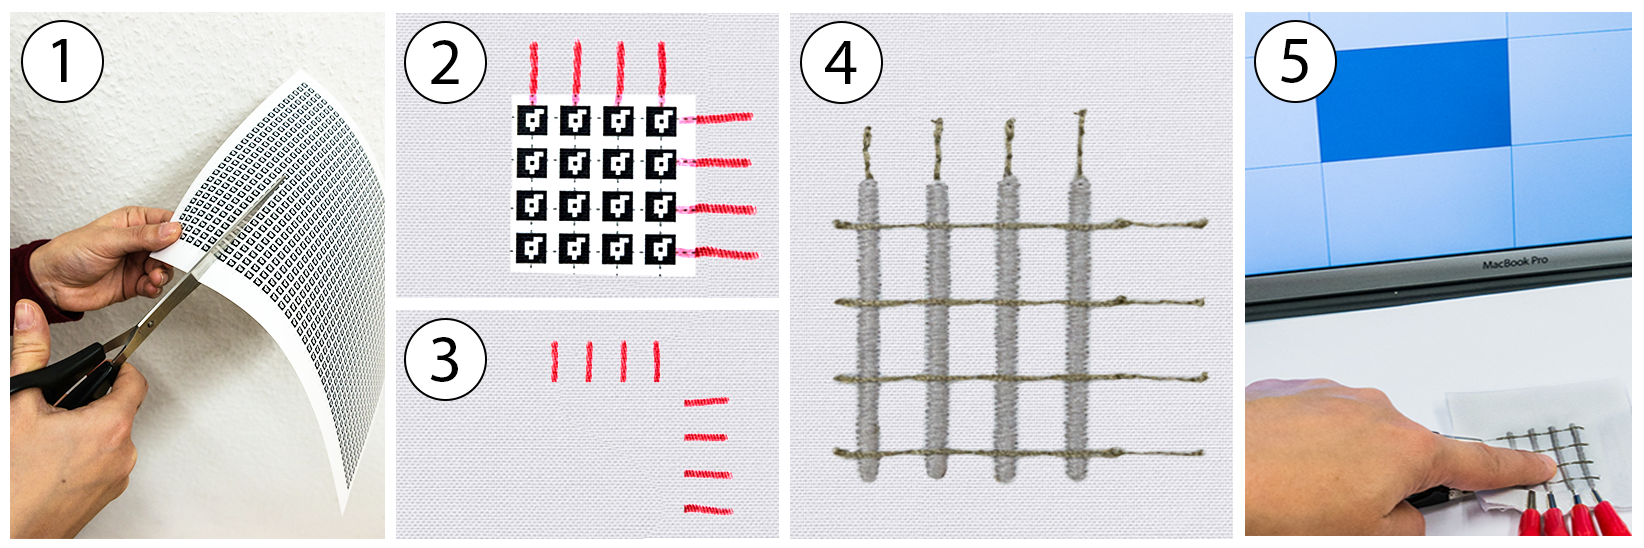
\includegraphics[width=1.0\columnwidth]{figures/Touchpad.png}
  \caption{Sensor Sticker process: 1. A user cuts the sticker, 2. adheres it to fabric, and draws connecting traces with \textit{trace color} pen, 3. captures the design and removes the sticker, 4. the system stitches the sensor.}~\label{fig:Touchpad}
  \vspace{-1.8em}
  \end{figure}

% To create a sensor in Sketch\&Stitch, the user prints the \textit{Sensor Sticker} on a sheet of adhesive paper, cuts it into the desired shape to create a slider or a touchpad, and sticks it onto the fabric, then draws connecting traces from two sensor grid edges to pins of a controller using the \textit{trace color} marker. After capturing the design, the user removes the \textit{Sensor Sticker}, and the embroidery machine stitches the sensor pattern in place. Fig.\ \ref{fig:Sensor} shows a 2D touchpad at different stages of the embroidery process to show the different layers.

% Electronically speaking, rectangular sensors are the easiest to create that way. The user connects to them at two of their adjacent edges. Other convex shapes require per-line calibration in software to account for the different lengths of grid lines, and concave shapes may also require multiple connections per line if it is interrupted, like the top row in Fig.\ \ref{fig:Sensor}.
% %The grid was designed based on the recommendation of Texas Instruments 


% constructed by “opening up” a capacitor structure so that the
% electric field can be interfered with by a conductive foreign object, in this case, a fingerWhen a conductor, e.g., a finger,
% comes into the area above the open capacitor, the electric field is interfered with causing the
% resulting capacitance to change. The coupling of the conductive finger into the capacitive sensor
% increases the capacitance of the structure beyond the baseline capacitance, the capacitance of
% the sensor with no touch. By continuously measuring the capacitance of the sensor(s) in the
% system and comparing each result to a predetermined baseline capacitance, the system
% microcontroller can determine not only on/off button functions for each sensor element but also
% “amount” of press used for more complex interfaces such as positional sliders. 
% The base capacitance of such a design is affected by stray capacitances on the PCB as well as
% potentially other environmental effects such as temperature and humidity. Therefore, the
% detection system needs to constantly monitor and track this variation for correct comparison to
% touch events. 



 

\subsection{Circuit Integration Strategies}
Our system offers five strategies to integrate circuit traces and hardware components in a design: the first is drawing circuit traces to be part of the artwork. The second is drawing circuit traces close to art outlines, which makes traces less obvious.
%The spacing constraint of 2.5 mm need not to be applied between conductive and non-conductive threads. 
%since the width of art stitches is relatively larger than trace stitches.
The third is camouflaging traces by insulating them with a thread color that matches the color of the base fabric \cite{Buechley2009}. %Traces will not be hidden completely, but depending on the desired application, this technique may be sufficient to occlude electrical connections. 
The fourth hides hardware components by attaching them to their contact area from the back side of fabric using one of the suggested thread-based attachment techniques. The fifth hides fabric circuits completely. It uses two layers of fabric: a top layer for the artwork, and a bottom layer for traces and Circuitry Stickers. The two fabrics are sketched and embroidered individually. At the end of embroidery, the user attaches components to the bottom fabric and manually layers the fabrics on top of each other. Capacitive touch sensors will work through a thin top fabric. For components that need to be visible on the surface, such as light sensors and LEDs, the user may cut openings into the top fabric. Another option is attach these parts on the top fabric and use thread-based attachment to connect them to their contact surface on the bottom layer. This technique can also be used to create multi-layer textile circuits \cite{Dunne:2012:MEC:2370216.2370348, 5387040}, with the addition of an insulator, like non-conductive fabric, between any two conductive layers. 

%*art colors focrecs the embroidery machine to pause for and wait for the user to chnage thread color. The machine itself can detect color in an image but cannot distigusih thread colors. 


   
   
\subsection{Debugging}
\begin{figure} [t!]
\centering
  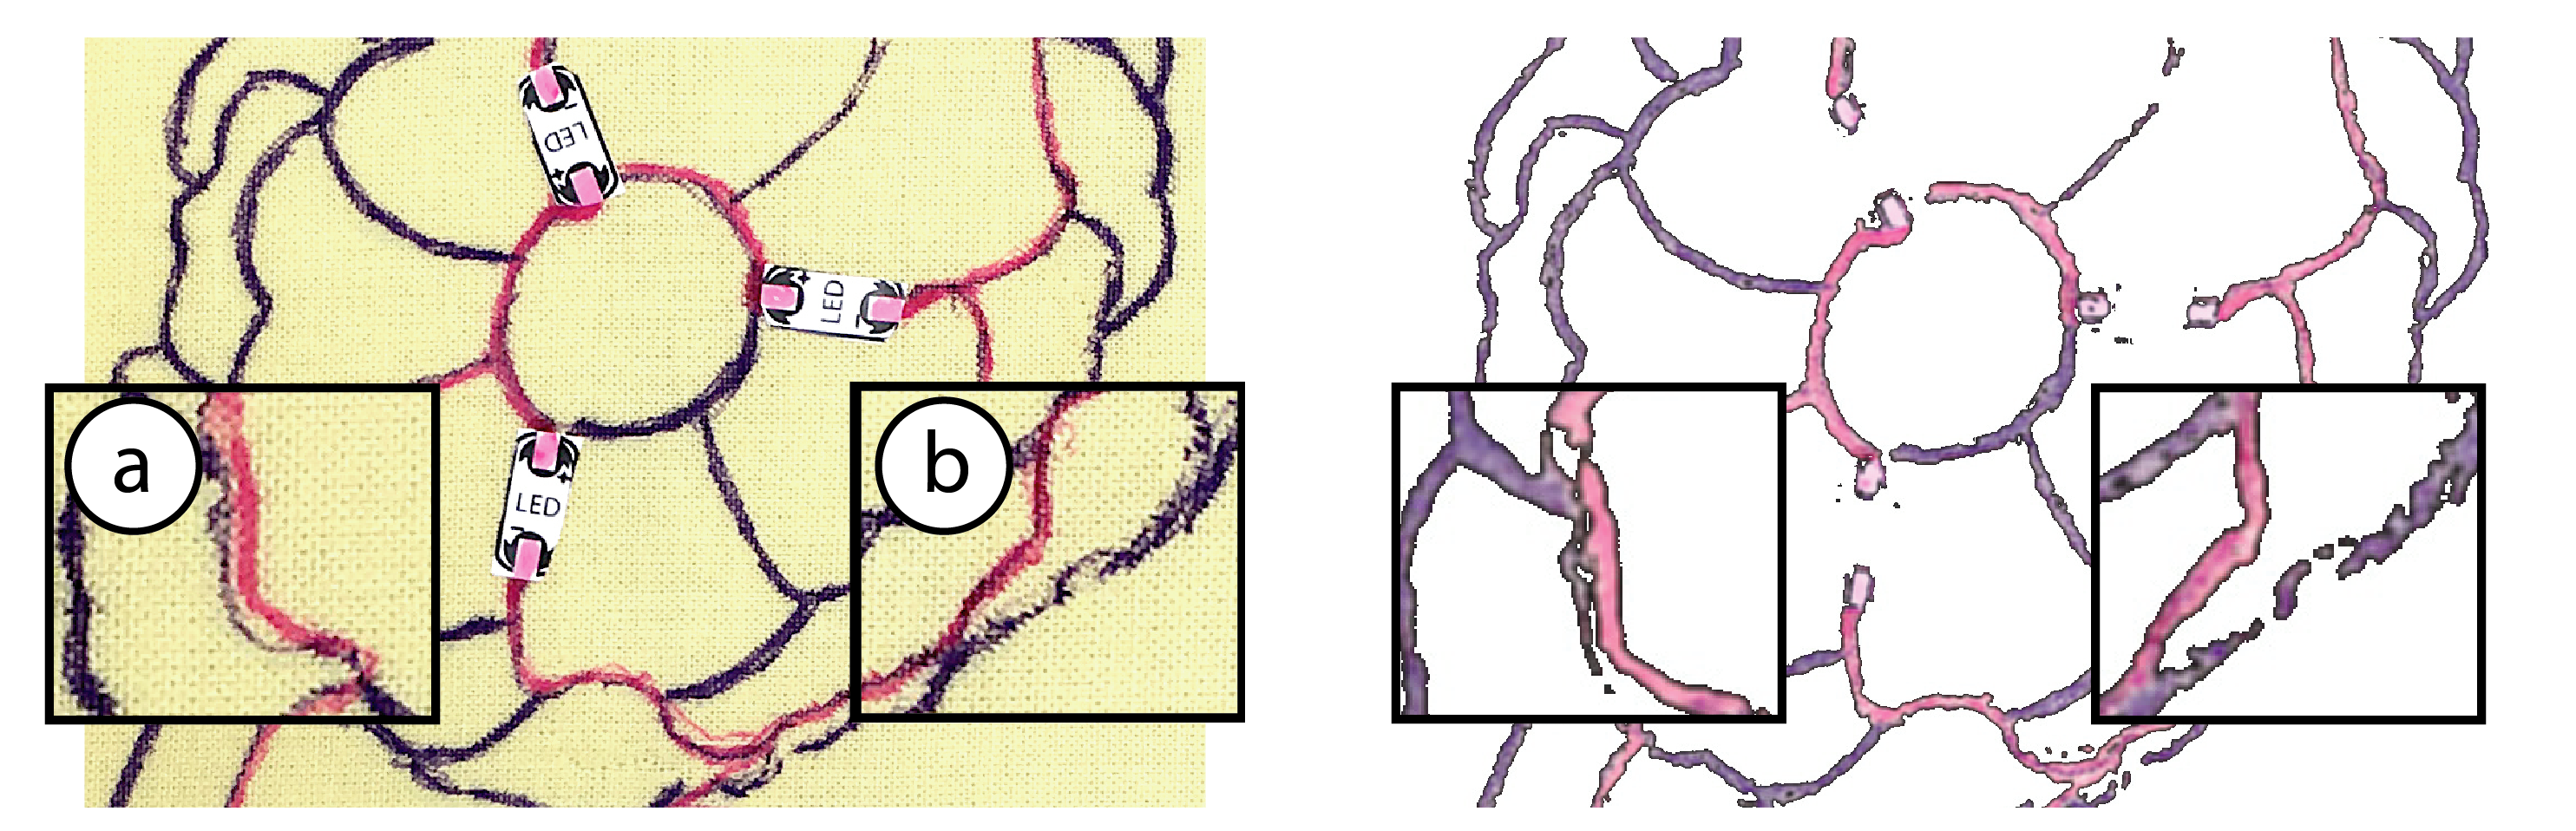
\includegraphics[width=0.9\columnwidth]{figures/Debugging.png}
  \caption{Sketch digitization pitfalls: a. Merged lines. b. Segmented lines.}~\label{fig:Debugging}
  \vspace{-2.2em}
\end{figure}
Users can debug their designs at three stages in the workflow. The system provides users with feedback to detect pitfalls, such as indistinguishable colors, segmented lines, and merged lines, from sketch digitization. After assigning the color palette, our S\&S PC app displays the detected colors on the PC screen. Based on this early feedback, the user decides to redo color assignment using, e.g., different pen colors, or to start sketching. Similarly, after each capture of the sketch, the app displays the digitized design on the PC screen. A mismatch between the design (input) and the preview (output) could be caused by poor lighting, shadows, indistinct strokes, color variability, or other artifacts commonly present in photographed images. Indistinct strokes and color variability occur due to pen jitters over textured fabrics and variable pressures applied while drawing a single stroke, causing the stroke color to vary between darker and lighter shades. Consequently, a trace may appear segmented during color detection, resulting in an open circuit in the final product. To handle these issues, the S\&S PC app offers an optional slider-based interface for manually tuning color detection. Otherwise, the user should perform the proper adjustments directly on the fabric, e.g., remove sources of shadow, or emphasize the strokes, and recapture her design. 

Once the sketch in converted to stitches, the user sees what the end result will look like via the embroidery machine's touch display (WYSIWYG editor). The display offers tools to zoom in, duplicate, mirror, translate, etc.\ the design as a whole, but it does not allow the user to change the design on the stitch level. Using this preview, the user can detect the issue of merged traces, which occurs when the spacing between two independent lines is less than 0.2 mm (see Technical Stitching). The user fixes this by erasing the problematic traces on fabric and re-sketching them further apart. Finally, the \textit{incremental design} feature allows her to test the physical design, artwork and circuit, by selectively sketching and stitching parts of it. She may also use another piece of fabric to stitch the first iteration before committing on the final fabric.


%Limitation, no feedback during sketching, no automatic detection of issues.
%Limitation no more 'adjustment options', e.g., on the stitch level, because they need more experience.
%The history of transformations can be accessed on the embroidery machine.



\section{Walkthrough: Interactive Flower}
\begin{figure} [t!]
\centering
  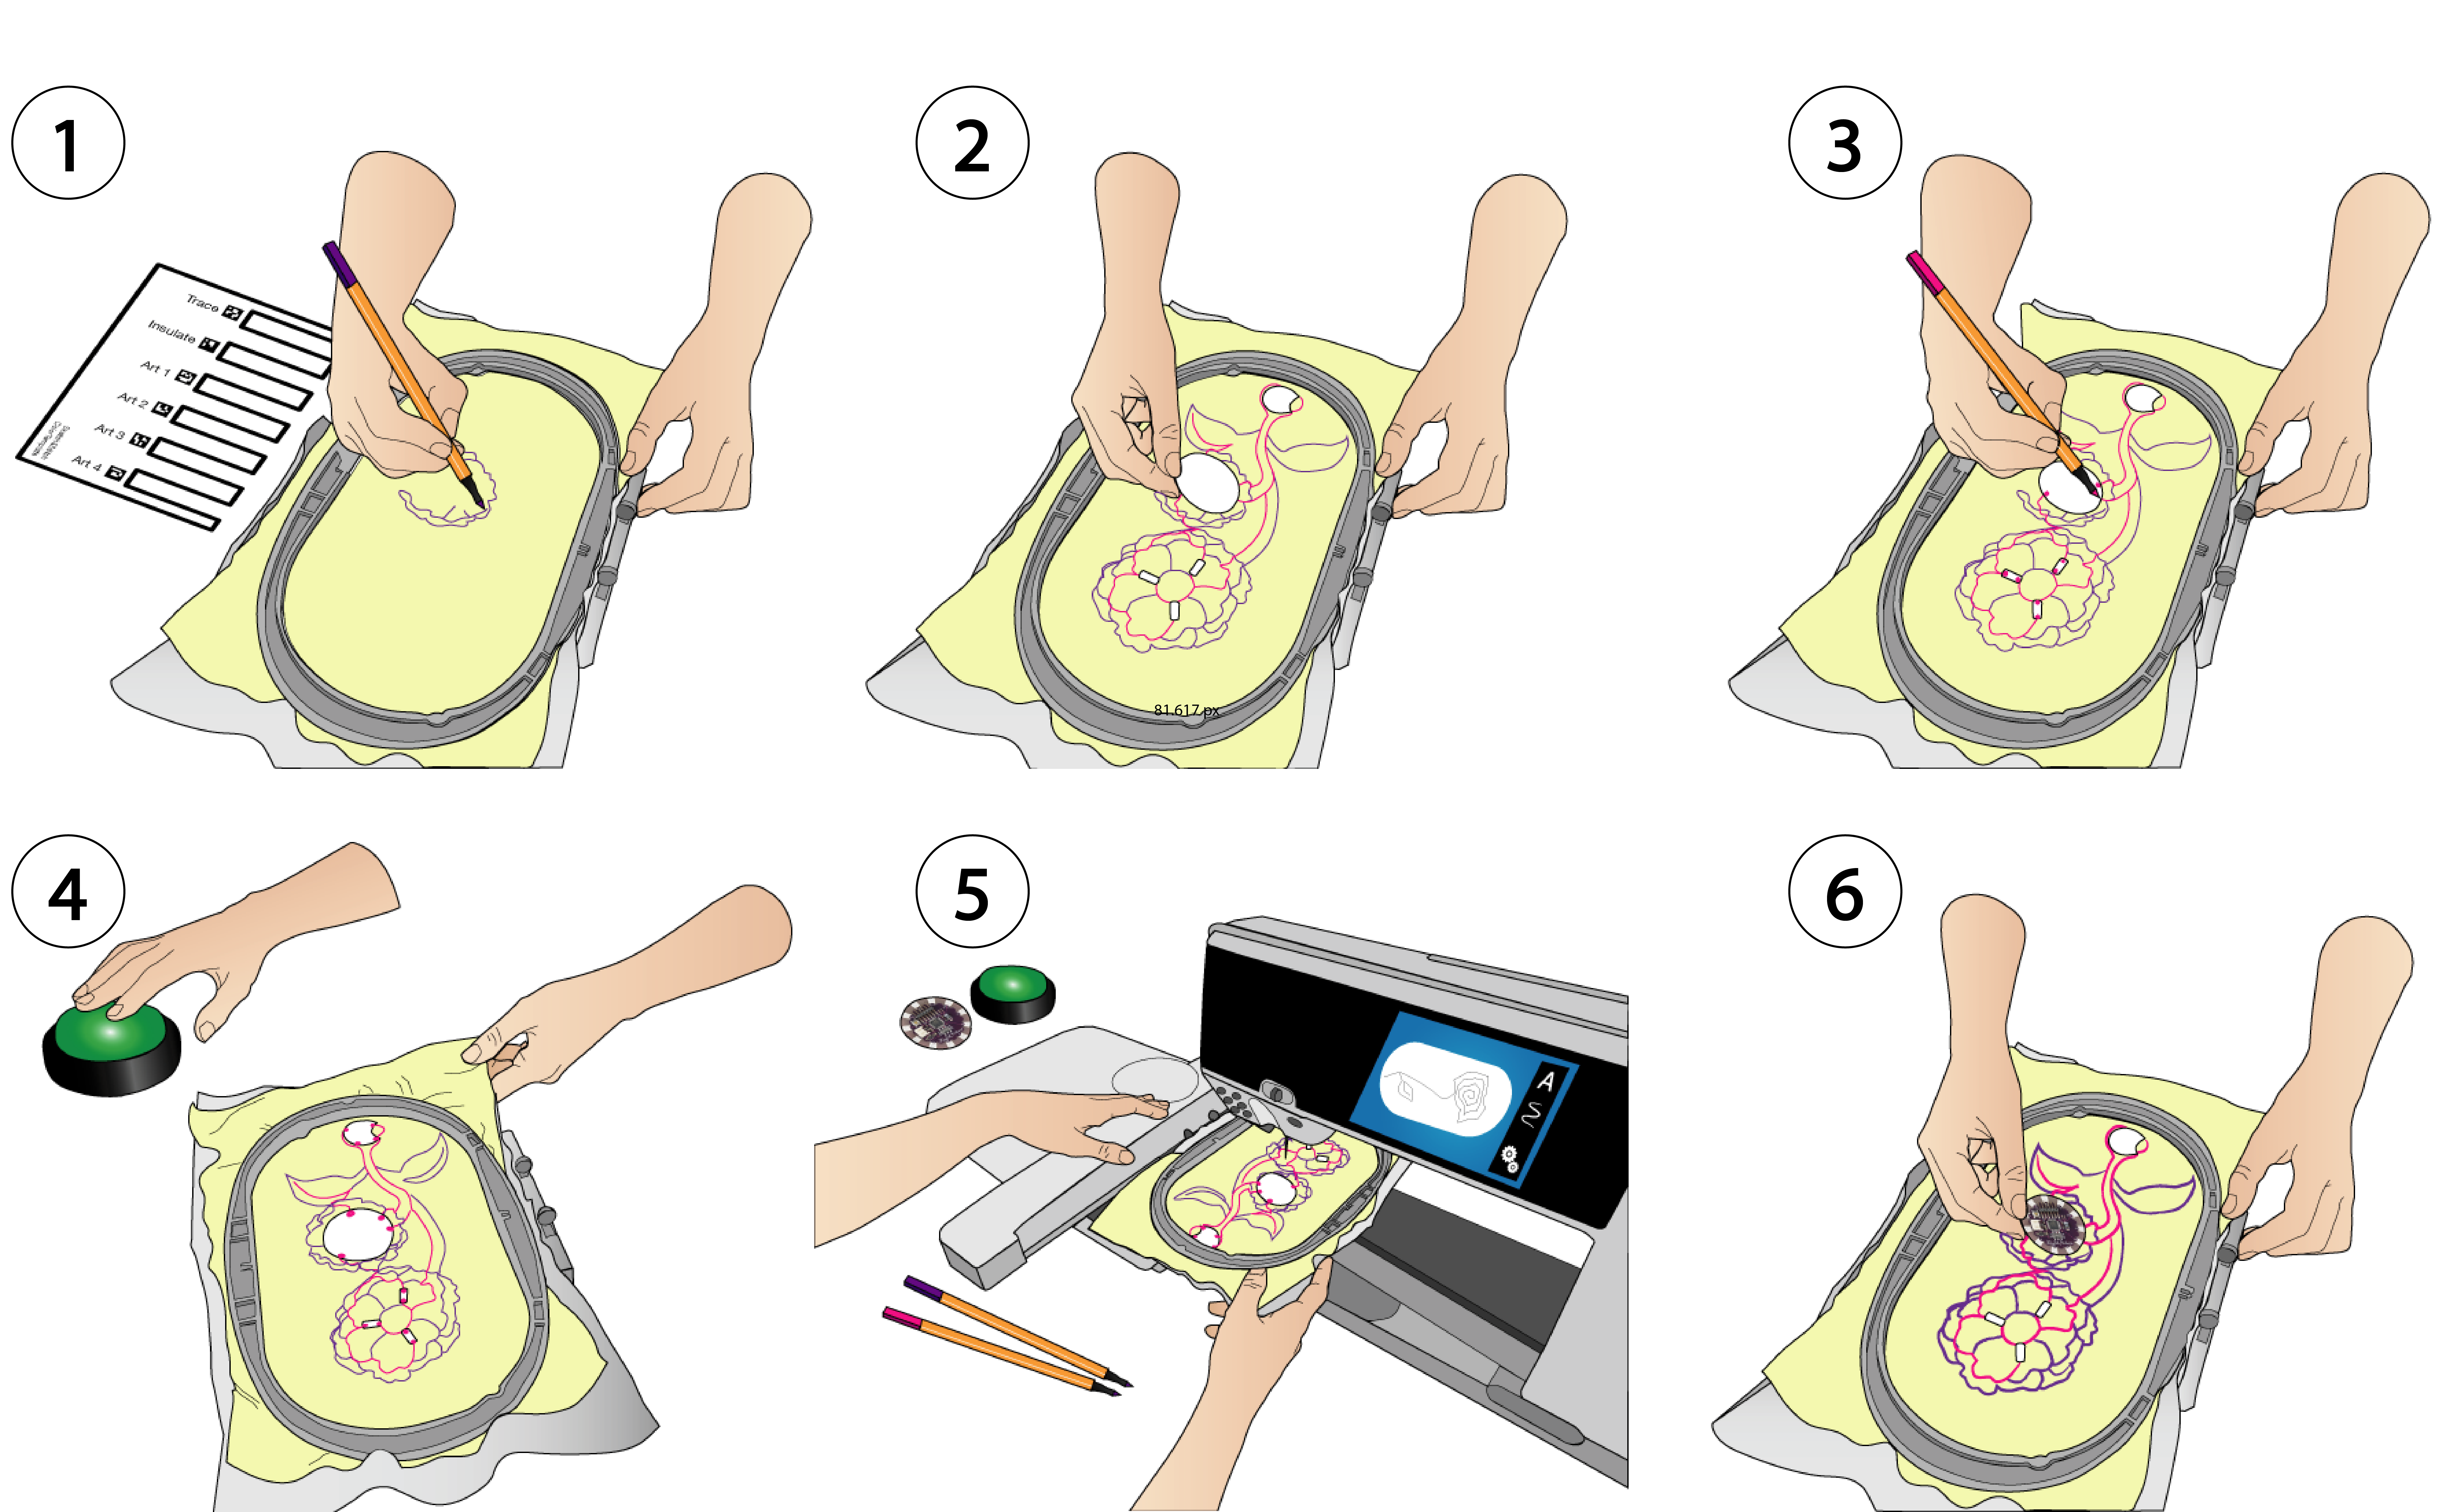
\includegraphics[width=0.9\columnwidth]{figures/Walkthrough.png}
  \caption{Basic workflow: 1. Sketch a design on fabric, 2. adhere Circuitry Stickers, 3. draw the circuit and electrical connections, 4. capture a picture of the sketch, 5. insert the fabric into the embroidery machine for stitching, and 6. replace the stickers with hardware components.}~\label{fig:Walkthrough}
  \vspace{-2.2em}
\end{figure}

We illustrate Sketch\&Stitch's basic workflow using the example of an interactive flower that emits light patterns when the user touches one of its leaves (Fig.\ \ref{fig:Walkthrough}). %The flower includes 3 LEDs, 1 battery holder, and 1 microcontroller 
%ATmega32U4 Board from the LilyPad kit. 


\textit{Sketching and Placing Circuitry Stickers}. To start, the user places the color template on her fabric and draws two strokes in the violet and pink pens in the trace and art slits, respectively. She captures a picture of the template, and confirms color detection on the PC screen. She hoops her fabric and starts drawing the outline of a flower using an \textit{art color} pen. She adheres a Component Sticker for a Lilypad controller on the fabric. She draws a trace from a pin on the sticker to the leaf of the flower using the \textit{trace color} pen, creating a capacitive pushbutton. She continues sketching and adding stickers.


\textit{Capturing and Stitching Design}. The user captures a picture of her sketch, and verifies the digitized design on the PC screen.
With no Embroidery Stickers to remove in her design, she secures the hoop in the embroidery machine and uses the embedded display to view the embroidery patterns of her design. She sees objects in \textit{trace color} sequenced to be stitched first. She threads the embroidery needle with conductive thread and starts stitching. Each time the machine finishes stitching one pattern, it pauses and prompts her to change threads. 
%The user picks a non-conductive thread of the color she wants for each part (red for the flower, green for the stem) and starts the machine again. 

\textit{Attaching Electronics}. After embroidery is complete, she removes the hoop from the machine, and trims jump stitches using scissors. She cuts off pieces of Z-tape and sticks them onto the back of her hardware components. Guided by the Component Stickers, she determines the location and orientation of each component. She replaces the stickers with the hardware. Finally, she uses the Arduino IDE to program the LilyPad. More
beginner-friendly tools exist, e.g. Scratch \cite{Resnick:2009:SP:1592761.1592779}. %The e-textile is complete.

%Finally, she inserts a battery into the battery holder and sees her design augmented with a touch-sensitive lightup effect. 




\section{Technical Stitching}
We used the Bernina 880B
%\footnote{www.bernina.com/880}
embroidery machine and its software, DesignerPlus v.8, with Shieldex 117/17 dtex 2-ply silver sewing thread (linear resistance < 30 $\Omega$/cm) as a top thread.
%http://www.shieldextrading.net/products/yarns-threads/
%This thread can carry current for power and signals. The embroidery machine requires two types of thread: 
%In embroidery machines, the top thread appears on the surface of the fabric, and the bobbin thread runs on the back side of the fabric to pull the top thread down. %Users can control the shape of the top thread but not the bobbin's. 
Embroidery is one of the most stressful textile processes for conductive thread \cite{5387040}. This leads to thread breaks and segmented circuit traces. A stitching speed of 700 stitch/min reduces the heat and friction associated with high speeds. %and used metallic thread needles.
%a light weight bobbin thread (60 wt).

Table \ref{tab:Stitches} summarizes the stitches that Sketch\&Stitch uses to embroider users' designs. The Satin stitch is used to stitch the artwork. The length of a stitch determines the margin of error in the length of sketched and insulated traces when stitched. 
%trace increases by 0--0.8 mm or by 0--0.3 mm for insulated traces when stitched. 
The width of a sketched line increases by 0--0.2 mm when stitched due to the smoothing algorithm that the embroidery software uses before transforming a digital sketch to embroidery patterns. Thus, gaps that are 0.2 mm wide between adjacent stokes may be closed with stitches. We describe three tests for determining the system's stitches. We compared variants of the basic stitch types, Satin, and Triple and Single Running. We excluded special purpose and decorative stitches. %The Satin stitch has a variable width, suitable for outlining lines and filling shapes. Running stitches have a fixed width and are only used for outlines. 
The tests were conducted on cotton and linen fabrics. Measurements were taken directly after embroidery, and after one and two weeks of frequent fabric handling. We report the average measurements.



  

\begin{table}[]
\centering
\resizebox{0.47\textwidth}{!}{
\begin{tabular}[]{lcccc}
\hline
Stitch & Trace & Insulation & Grid &Bridge  \\ \hline
Type &Satin & Satin & Triple & Triple \\
Length & 0.8 mm & 0.3 mm & 1.0-2.5 mm  & 9.0 mm \\
Width & 1.0+ mm & 1.8 mm & 1.0 mm & 1.0 mm \\
Purpose & \begin{tabular}[t]{c} Sketched \\ traces\end{tabular} & Insulation & \begin{tabular}[t]{c}Insulated traces\\ Sensor traces\end{tabular} & Shield bridges \\
Shape & \multicolumn{2}{l}{\parbox[]{}{
  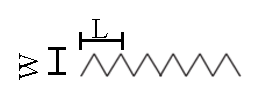
\includegraphics[width=1in]{figures/satin_shape}}} & \multicolumn{1}{l}{\parbox[l]{1em}{
  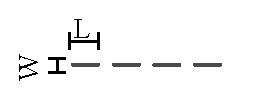
\includegraphics[width=1in]{figures/running_shape}}} &
  \multicolumn{1}{l}{\parbox[l]{1em}{
  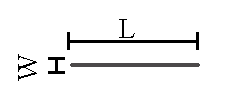
\includegraphics[width=1in]{figures/bridge_shape}}} \\
\hline
\end{tabular}%
}
\caption{Technical stitches for embroidering fabric traces and sensors.}
\label{tab:Stitches}
\vspace{-1.2em}
\end{table} 

%Single and and Triple Running are forward stitches, the latter uses three overlapping threads per stitch instead of one.

%Step stitch can also be used as a basic filling stitch, but Satin produces more appealing results.


%---> FW: Need more experiments to understand the effect of thread types (e.g., Madeira), time (aging), base fabric types, on resistance, spacing, and couching 

 \subsection{Resisitivity Test} 
 Fabric circuits with long electrical connections drop significantly more voltage, consuming power and limiting the amount of current that can be delivered to components. To determine the \textit{trace stitch} for hand-sketched traces, we measured the resistance of 30 conductive traces: \textsc{trace length} (5 cm and 10 cm) $\times$ \textsc{stitch type} (Satin, Triple, Single) $\times$ \textsc{stitch length} (0.4, 0.6, 0.8, 1.0, 2.0 mm), all with minimum width. Table \ref{tab:Resistance} shows sample traces and their average measured resistance. Overall, the resistance of Satin traces was lower than Running traces, independent of \textsc{stitch length}. Satin traces of shorter \textsc{stitch lengths} measured marginally lower resistances. But as the stitch length became shorter, traces became denser. This affects the flexibility of the base fabric, especially if several traces are concentrated in a small area. Longer stitches result in spars traces. Consequently, we chose the Satin stitch of 0.8 mm length as the \textit{trace stitch}.  The \textit{grid stitch} is used for stitching insulated traces and sticker sensor traces. As these traces will be covered with an \textit{insulation stitch}, and are often concentrated in a small area, it is essential for them to be flexible. We chose the Triple stitch with an adaptable length of 1--2.5 mm as the \textit{grid stitch}.

\begin{table}[h] 
\centering
\resizebox{0.47\textwidth}{!}{
\begin{tabular}{lccl} 
  \hline 
  Stitch Type & Stitch Length & Resistance & Sample \hspace{15mm} \\
  \hline  Satin & 0.4 mm & 5--12\Omega & \parbox[c]{1em}{
  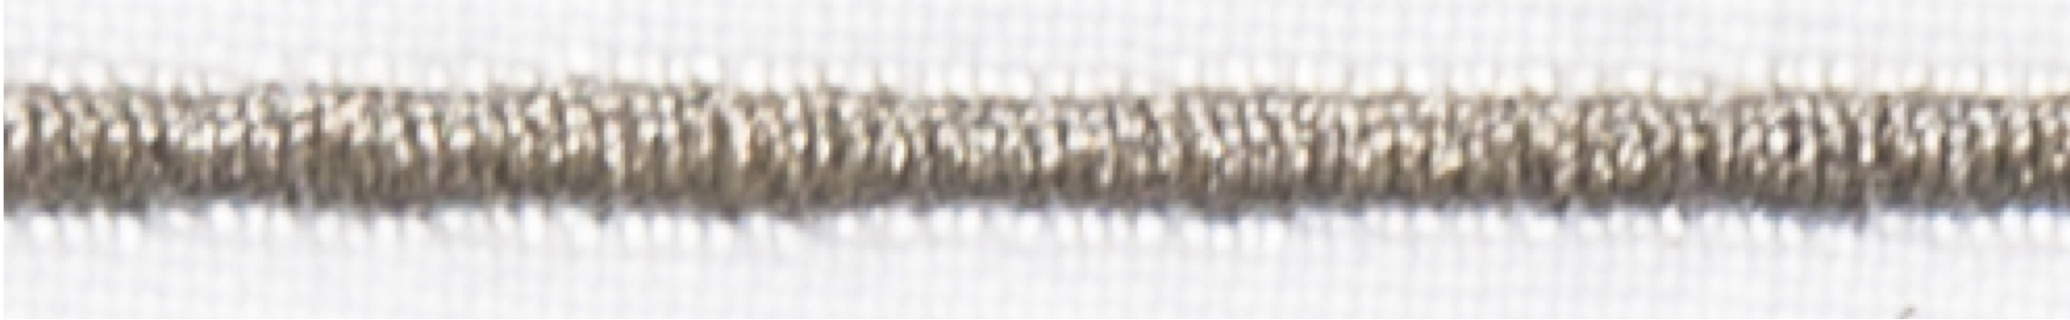
\includegraphics[width=1in]{figures/satin04}} \\
    Satin & 0.6 mm & 12--15 \Omega & \parbox[c]{1em}{
  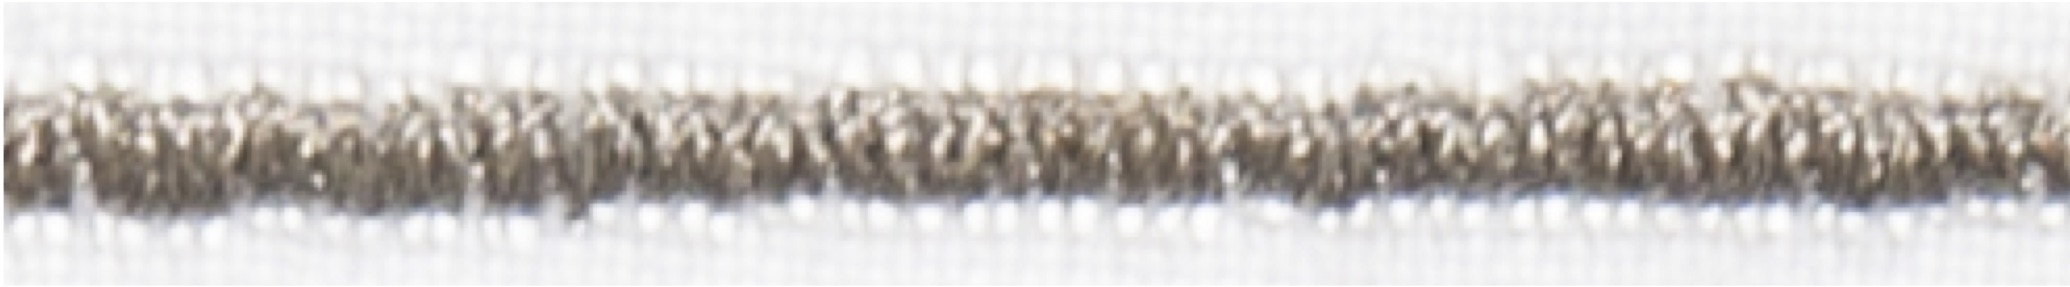
\includegraphics[width=1in]{figures/satin06}} \\
    Satin & 2.0 mm & 14--20 \Omega & \parbox[c]{1em}{
  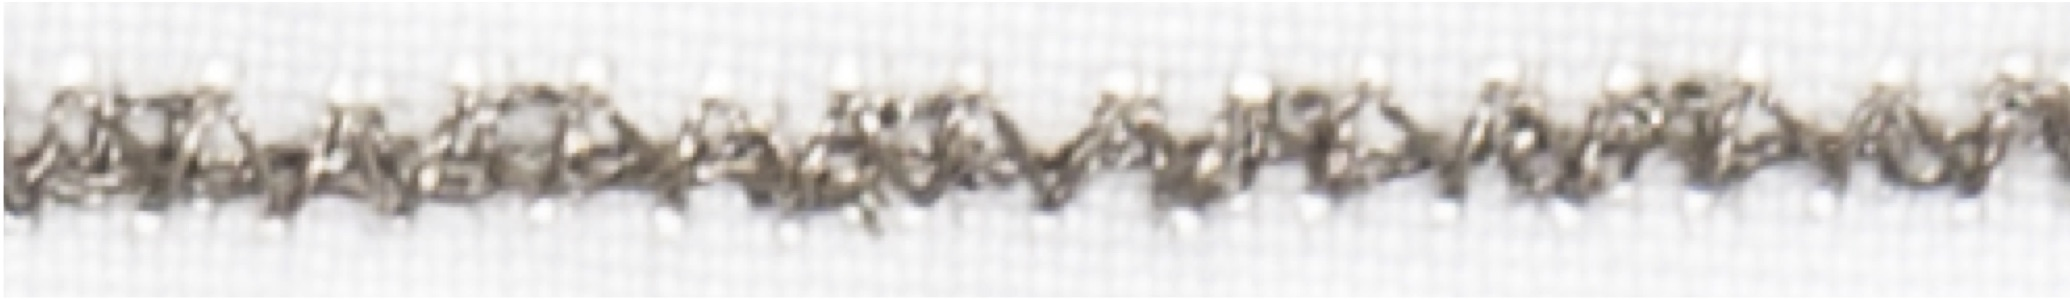
\includegraphics[width=1in]{figures/satin20}} \\
   Triple & 2.0 mm & 27--53 \Omega & \parbox[c]{1em}{
  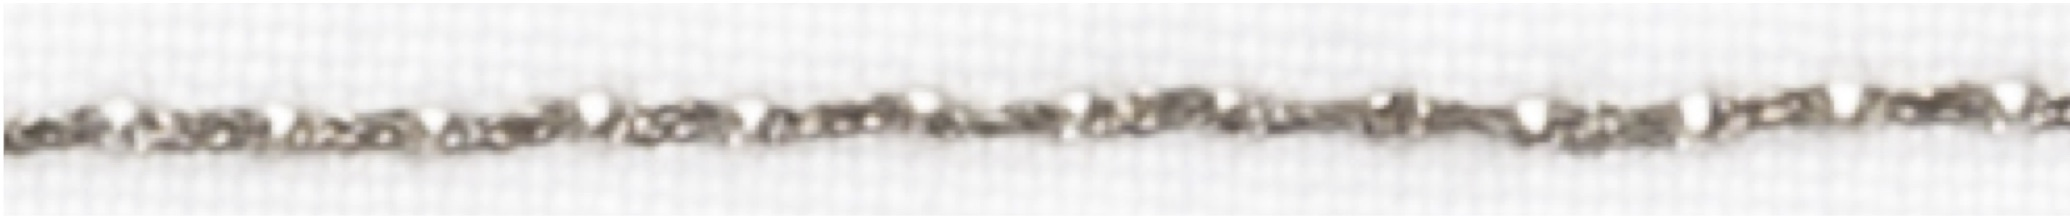
\includegraphics[width=1in]{figures/triple20}} \\
    Single & 2.0 mm & 31--80 \Omega & \parbox[c]{1em}{
  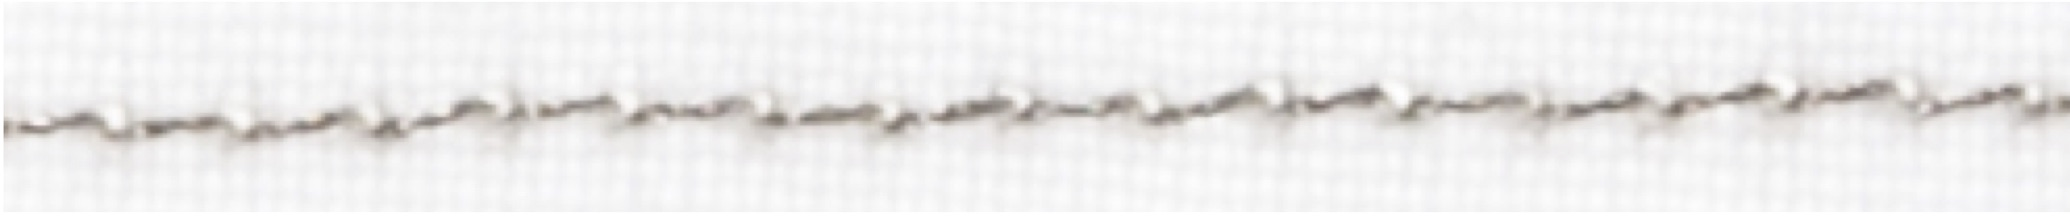
\includegraphics[width=1in]{figures/single20}} \\
   \hline
\end{tabular}
}
\caption{A sample of conductive traces stitched with Satin and Running stitches, and their measured resistance for 5 and 10 cm long segments.}
\label{tab:Resistance}
\vspace{-1em}
\end{table}

%Unlike traditional copper wires, conductive threads have relatively high resistances. Resistive threads can be desired for some applications, e.g., \cite{Gowrishankar:2013:PRE:2493988.2494341}. 

%denser stitches increase the number of connections between the conductive fibers that compose a thread, reducing the trace resistance 

\subsection{Spacing Test} 
To evaluate the smallest pitch achievable in our touchpad sensor, we tested the minimum allowed spacing between parallel exposed traces to avoid undesired connections. We measured for continuity between 6 conductive traces, stitched with the \textit{grid stitch}, and separated by different \textsc{Spacings} (1.0, 1.5, 2.0, 2.5, 3.0, 3.5 mm). Fraying fibers connected traces at 1.0 and 1.5 mm distances. At 2 mm distance, tie-in and tie-off knots, which are often wider than the trace itself, created undesired contacts on the back of fabric. We conclude that a 2.5 mm is the safe minimum distance between exposed traces. These results are independent of the type, length, and width of a stitch, but may differ for other types of conductive thread. %with variant fiber lengths. 

\subsection{Insulation Test}
Our goal was to find an \textit{insulation stitch} that prevents undesired connections to occur between insulated and exposed traces even if they come in direct contact with each other, such as in shields and sensors. The most common couch stitch is the Satin (Zigzag) stitch. 
 We tested 16 conductive traces, 10 cm long, stitched with the \textit{grid stitch} and couched with a Satin stitch: \textsc{stitch width} (1.0, 1.5, 2.0, 2.5 mm) $\times$ \textsc{stitch length} (0.7, 0.5, 0.3, 0.1 mm). Each insulated trace was pressed against an exposed conductive trace with four amounts of \textsc{pressure} (1, 5, 15, 30 N) at 5 equidistant points along the trace. We measured for continuity. Fig.\ \ref{fig:Insulation} summarizes the results. We found that the Satin stitch of 1.5 mm width and 0.3 mm length insulates a conductive trace on both sides of the fabric while having the least effect on base fabric flexibility. Thus, two insulated traces can be spaced as close as 2 mm---closer than exposed ones.


\begin{figure}[t!]
\vspace{-1em}
    \centering
    \resizebox{0.49\textwidth}{!}{
        % Created by tikzDevice version 0.10.1 on 2018-01-06 23:58:38
% !TEX encoding = UTF-8 Unicode
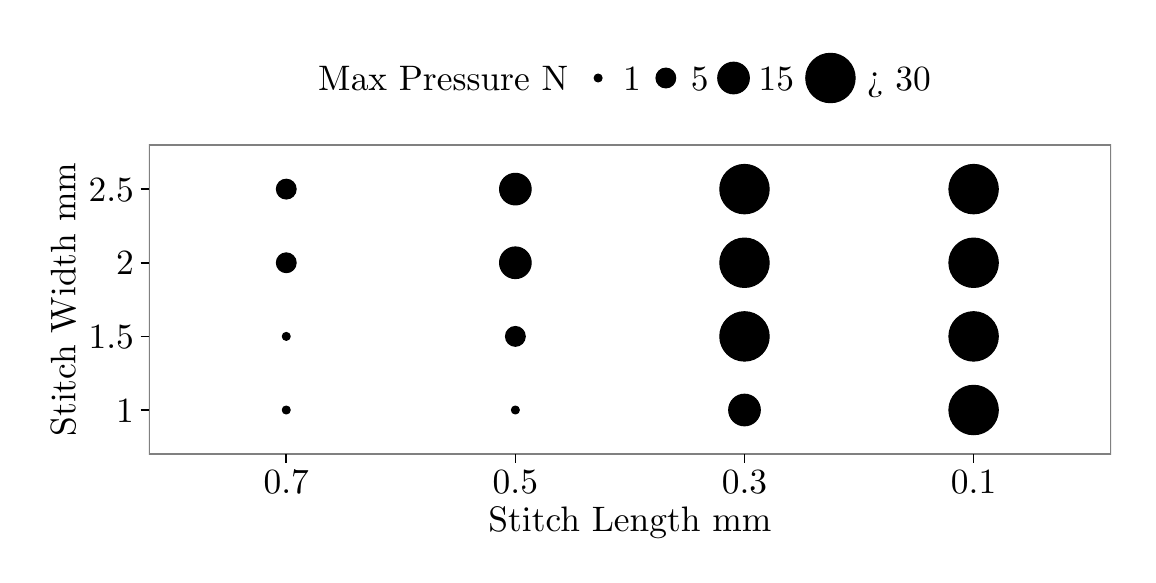
\begin{tikzpicture}[x=1pt,y=1pt]
\definecolor{fillColor}{RGB}{255,255,255}
\path[use as bounding box,fill=fillColor,fill opacity=0.00] (0,0) rectangle (397.48,190.36);
\begin{scope}
\path[clip] (  0.00,  0.00) rectangle (397.48,190.36);
\definecolor{drawColor}{RGB}{255,255,255}
\definecolor{fillColor}{RGB}{255,255,255}

\path[draw=drawColor,line width= 0.6pt,line join=round,line cap=round,fill=fillColor] (  0.00, -0.00) rectangle (397.48,202.36);
\end{scope}
\begin{scope}
\path[clip] ( 43.77, 36.23) rectangle (391.48,147.99);
\definecolor{fillColor}{RGB}{255,255,255}

\path[fill=fillColor] ( 43.77, 36.23) rectangle (391.48,147.99);
\definecolor{drawColor}{RGB}{0,0,0}
\definecolor{fillColor}{RGB}{0,0,0}

\path[draw=drawColor,line width= 0.4pt,line join=round,line cap=round,fill=fillColor] (341.81, 52.20) circle (  8.92);

\path[draw=drawColor,line width= 0.4pt,line join=round,line cap=round,fill=fillColor] (341.81, 78.80) circle (  8.92);

\path[draw=drawColor,line width= 0.4pt,line join=round,line cap=round,fill=fillColor] (341.81,105.41) circle (  8.92);

\path[draw=drawColor,line width= 0.4pt,line join=round,line cap=round,fill=fillColor] (341.81,132.02) circle (  8.92);

\path[draw=drawColor,line width= 0.4pt,line join=round,line cap=round,fill=fillColor] (259.02, 52.20) circle (  5.71);

\path[draw=drawColor,line width= 0.4pt,line join=round,line cap=round,fill=fillColor] (259.02, 78.80) circle (  8.92);

\path[draw=drawColor,line width= 0.4pt,line join=round,line cap=round,fill=fillColor] (259.02,105.41) circle (  8.92);

\path[draw=drawColor,line width= 0.4pt,line join=round,line cap=round,fill=fillColor] (259.02,132.02) circle (  8.92);

\path[draw=drawColor,line width= 0.4pt,line join=round,line cap=round,fill=fillColor] (176.23, 52.20) circle (  1.43);

\path[draw=drawColor,line width= 0.4pt,line join=round,line cap=round,fill=fillColor] (176.23, 78.80) circle (  3.57);

\path[draw=drawColor,line width= 0.4pt,line join=round,line cap=round,fill=fillColor] (176.23,105.41) circle (  5.71);

\path[draw=drawColor,line width= 0.4pt,line join=round,line cap=round,fill=fillColor] (176.23,132.02) circle (  5.71);

\path[draw=drawColor,line width= 0.4pt,line join=round,line cap=round,fill=fillColor] ( 93.44, 52.20) circle (  1.43);

\path[draw=drawColor,line width= 0.4pt,line join=round,line cap=round,fill=fillColor] ( 93.44, 78.80) circle (  1.43);

\path[draw=drawColor,line width= 0.4pt,line join=round,line cap=round,fill=fillColor] ( 93.44,105.41) circle (  3.57);

\path[draw=drawColor,line width= 0.4pt,line join=round,line cap=round,fill=fillColor] ( 93.44,132.02) circle (  3.57);
\definecolor{drawColor}{gray}{0.50}

\path[draw=drawColor,line width= 0.6pt,line join=round,line cap=round] ( 43.77, 36.23) rectangle (391.48,147.99);
\end{scope}
\begin{scope}
\path[clip] (  0.00,  0.00) rectangle (397.48,202.36);
\definecolor{drawColor}{RGB}{0,0,0}

\node[text=drawColor,anchor=base east,inner sep=0pt, outer sep=0pt, scale=  1.28] at ( 38.37, 47.79) {1};

\node[text=drawColor,anchor=base east,inner sep=0pt, outer sep=0pt, scale=  1.28] at ( 38.37, 74.40) {1.5};

\node[text=drawColor,anchor=base east,inner sep=0pt, outer sep=0pt, scale=  1.28] at ( 38.37,101.01) {2};

\node[text=drawColor,anchor=base east,inner sep=0pt, outer sep=0pt, scale=  1.28] at ( 38.37,127.61) {2.5};
\end{scope}
\begin{scope}
\path[clip] (  0.00,  0.00) rectangle (397.48,202.36);
\definecolor{drawColor}{RGB}{0,0,0}

\path[draw=drawColor,line width= 0.6pt,line join=round] ( 40.77, 52.20) --
	( 43.77, 52.20);

\path[draw=drawColor,line width= 0.6pt,line join=round] ( 40.77, 78.80) --
	( 43.77, 78.80);

\path[draw=drawColor,line width= 0.6pt,line join=round] ( 40.77,105.41) --
	( 43.77,105.41);

\path[draw=drawColor,line width= 0.6pt,line join=round] ( 40.77,132.02) --
	( 43.77,132.02);
\end{scope}
\begin{scope}
\path[clip] (  0.00,  0.00) rectangle (397.48,202.36);
\definecolor{drawColor}{RGB}{0,0,0}

\path[draw=drawColor,line width= 0.6pt,line join=round] ( 93.44, 33.23) --
	( 93.44, 36.23);

\path[draw=drawColor,line width= 0.6pt,line join=round] (176.23, 33.23) --
	(176.23, 36.23);

\path[draw=drawColor,line width= 0.6pt,line join=round] (259.02, 33.23) --
	(259.02, 36.23);

\path[draw=drawColor,line width= 0.6pt,line join=round] (341.81, 33.23) --
	(341.81, 36.23);
\end{scope}
\begin{scope}
\path[clip] (  0.00,  0.00) rectangle (397.48,202.36);
\definecolor{drawColor}{RGB}{0,0,0}

\node[text=drawColor,anchor=base,inner sep=0pt, outer sep=0pt, scale=  1.28] at ( 93.44, 22.02) {0.7};

\node[text=drawColor,anchor=base,inner sep=0pt, outer sep=0pt, scale=  1.28] at (176.23, 22.02) {0.5};

\node[text=drawColor,anchor=base,inner sep=0pt, outer sep=0pt, scale=  1.28] at (259.02, 22.02) {0.3};

\node[text=drawColor,anchor=base,inner sep=0pt, outer sep=0pt, scale=  1.28] at (341.81, 22.02) {0.1};
\end{scope}
\begin{scope}
\path[clip] (  0.00,  0.00) rectangle (397.48,202.36);
\definecolor{drawColor}{RGB}{0,0,0}

\node[text=drawColor,anchor=base,inner sep=0pt, outer sep=0pt, scale=  1.28] at (217.63,  8.40) {Stitch Length mm};
\end{scope}
\begin{scope}
\path[clip] (  0.00,  0.00) rectangle (397.48,202.36);
\definecolor{drawColor}{RGB}{0,0,0}

\node[text=drawColor,rotate= 90.00,anchor=base,inner sep=0pt, outer sep=0pt, scale=  1.28] at ( 17.22, 92.11) {Stitch Width mm};
\end{scope}
\begin{scope}
\path[clip] (  0.00,  0.00) rectangle (397.48,202.36);
\definecolor{fillColor}{RGB}{255,255,255}

\path[fill=fillColor] (100.70,156.52) rectangle (334.55,187.82);
\end{scope}
\begin{scope}
\path[clip] (  0.00,  0.00) rectangle (397.48,202.36);
\definecolor{drawColor}{RGB}{0,0,0}

\node[text=drawColor,anchor=base west,inner sep=0pt, outer sep=0pt, scale=  1.28] at (104.97,167.76) {Max Pressure N};
\end{scope}
\begin{scope}
\path[clip] (  0.00,  0.00) rectangle (397.48,202.36);
\definecolor{drawColor}{RGB}{255,255,255}
\definecolor{fillColor}{RGB}{255,255,255}

\path[draw=drawColor,line width= 0.6pt,line join=round,line cap=round,fill=fillColor] (198.90,160.79) rectangle (213.36,183.55);
\end{scope}
\begin{scope}
\path[clip] (  0.00,  0.00) rectangle (397.48,202.36);
\definecolor{drawColor}{RGB}{0,0,0}
\definecolor{fillColor}{RGB}{0,0,0}

\path[draw=drawColor,line width= 0.4pt,line join=round,line cap=round,fill=fillColor] (206.13,172.17) circle (  1.43);
\end{scope}
\begin{scope}
\path[clip] (  0.00,  0.00) rectangle (397.48,202.36);
\definecolor{drawColor}{RGB}{255,255,255}
\definecolor{fillColor}{RGB}{255,255,255}

\path[draw=drawColor,line width= 0.6pt,line join=round,line cap=round,fill=fillColor] (223.37,160.79) rectangle (237.82,183.55);
\end{scope}
\begin{scope}
\path[clip] (  0.00,  0.00) rectangle (397.48,202.36);
\definecolor{drawColor}{RGB}{0,0,0}
\definecolor{fillColor}{RGB}{0,0,0}

\path[draw=drawColor,line width= 0.4pt,line join=round,line cap=round,fill=fillColor] (230.60,172.17) circle (  3.57);
\end{scope}
\begin{scope}
\path[clip] (  0.00,  0.00) rectangle (397.48,202.36);
\definecolor{drawColor}{RGB}{255,255,255}
\definecolor{fillColor}{RGB}{255,255,255}

\path[draw=drawColor,line width= 0.6pt,line join=round,line cap=round,fill=fillColor] (247.84,160.79) rectangle (262.29,183.55);
\end{scope}
\begin{scope}
\path[clip] (  0.00,  0.00) rectangle (397.48,202.36);
\definecolor{drawColor}{RGB}{0,0,0}
\definecolor{fillColor}{RGB}{0,0,0}

\path[draw=drawColor,line width= 0.4pt,line join=round,line cap=round,fill=fillColor] (255.06,172.17) circle (  5.71);
\end{scope}
\begin{scope}
\path[clip] (  0.00,  0.00) rectangle (397.48,202.36);
\definecolor{drawColor}{RGB}{255,255,255}
\definecolor{fillColor}{RGB}{255,255,255}

\path[draw=drawColor,line width= 0.6pt,line join=round,line cap=round,fill=fillColor] (278.70,160.79) rectangle (301.46,183.55);
\end{scope}
\begin{scope}
\path[clip] (  0.00,  0.00) rectangle (397.48,202.36);
\definecolor{drawColor}{RGB}{0,0,0}
\definecolor{fillColor}{RGB}{0,0,0}

\path[draw=drawColor,line width= 0.4pt,line join=round,line cap=round,fill=fillColor] (290.08,172.17) circle (  8.92);
\end{scope}
\begin{scope}
\path[clip] (  0.00,  0.00) rectangle (397.48,202.36);
\definecolor{drawColor}{RGB}{0,0,0}

\node[text=drawColor,anchor=base west,inner sep=0pt, outer sep=0pt, scale=  1.28] at (215.17,167.76) {1};
\end{scope}
\begin{scope}
\path[clip] (  0.00,  0.00) rectangle (397.48,202.36);
\definecolor{drawColor}{RGB}{0,0,0}

\node[text=drawColor,anchor=base west,inner sep=0pt, outer sep=0pt, scale=  1.28] at (239.63,167.76) {5};
\end{scope}
\begin{scope}
\path[clip] (  0.00,  0.00) rectangle (397.48,202.36);
\definecolor{drawColor}{RGB}{0,0,0}

\node[text=drawColor,anchor=base west,inner sep=0pt, outer sep=0pt, scale=  1.28] at (264.10,167.76) {15};
\end{scope}
\begin{scope}
\path[clip] (  0.00,  0.00) rectangle (397.48,202.36);
\definecolor{drawColor}{RGB}{0,0,0}

\node[text=drawColor,anchor=base west,inner sep=0pt, outer sep=0pt, scale=  1.28] at (303.27,167.76) {> 30};
\end{scope}
\end{tikzpicture}

    }
    \caption{A plot of the relation between the width and length of Satin stitches and the max pressure under which they can insulate a trace.}
    \label{fig:Insulation}
    \vspace{-1.2em}
\end{figure}


\section{Implementation}
 \begin{figure}[h!]
\centering
  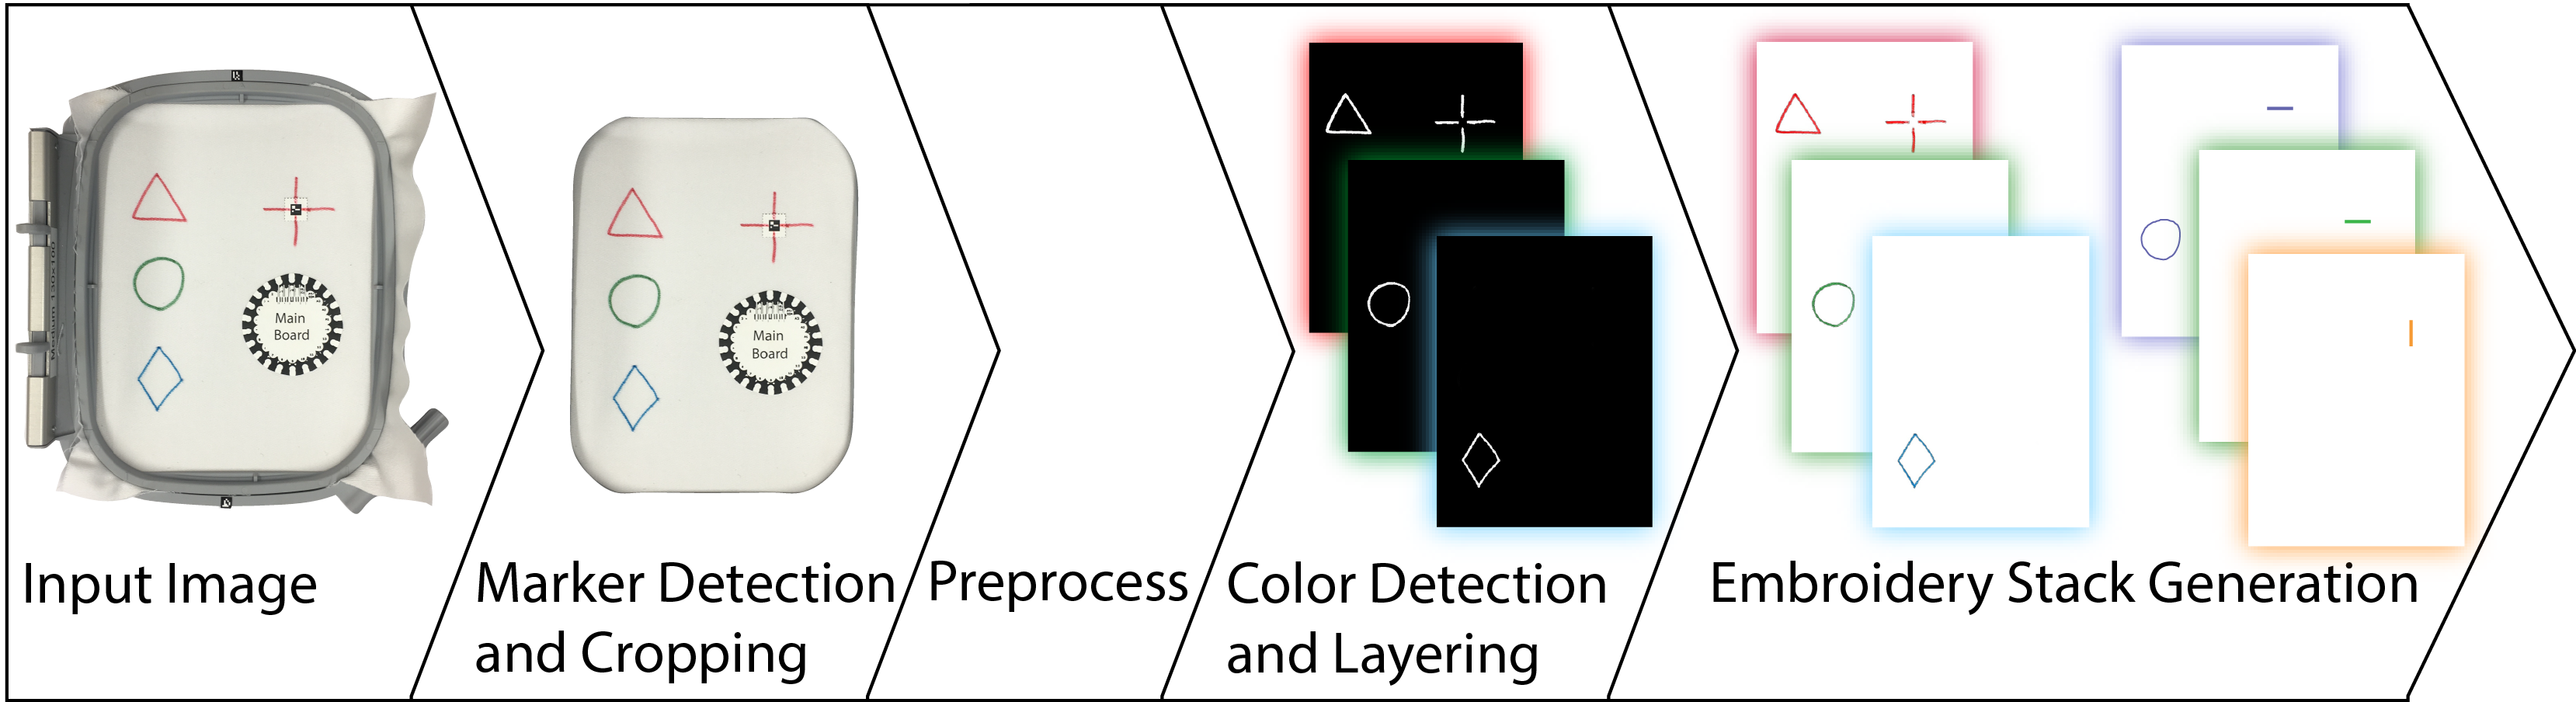
\includegraphics[width=1.0\columnwidth]{figures/Pipeline}
  \caption{Sketch digitization pipeline. Input image with the palette: red trace, green insulation, blue art, and a Shield and Component Stickers. Output embroidery stack excludes stickers, separates shapes in single-color layer, and generates two system layers: grid and bridge.}~\label{fig:Pipeline}
  \vspace{-1.2em}
  \end{figure}

\begin{figure*}[t!]
\centering
\includegraphics[width=1\textwidth]{figures/Applications.png}
\caption{Example applications: a. Wearable Mandala, b. Interactive Desk Mat, c. One-Hour Nap Pillow.}
 \vspace{-1.2em}
\label{fig:Applications}
\end{figure*}

\subfile{Implementation}




\section{Example Applications Created By an Artist} % and Emerging Design processes
To reveal early opportunities and challenges in Sketch\&Stitch workflow, we invited an artist with a technical background (female, 24 years old) to create e-textiles using our system over the course of three days. On the first day, the artist received a twenty-minute introduction of the system. For the next four hours, she practiced sketching and stitching simple shapes and basic circuits. In the following two days, she spent a total of 10 hours of unrestricted creative work. We observed and documented her process and artifacts, conducted 2 unstructured interviews (day 1 and 2) and a retrospective study with her and a researcher reviewing photos of her progress (day 3).

Below, we describe three unique e-textiles that were developed by the artist. She used the LilyPad hardware kit, which she programmed with the Arduino IDE. We follow this with a brief summary of her feedback and emerging processes. 

%we interviewed her to understand the design process that emerged while using our system. We describe these processes after the examples.

%\teaser{


\subsection{Wearable Mandala}
% \begin{figure} [h!]
% \centering
%   \includegraphics[width=1\columnwidth]{figures/Mandala} 
%   \caption{Example 1: The Wearable Mandala. Size 150$\times$150 mm, 20,000 stitches, 4 thread changes, 28 minutes stitch duration.}~\label{fig:Mandala}
%   \vspace{-1.5em}
% \end{figure}
%The first example is a wearable application. 
The artist sketched a mandala (150$\times$150 mm) on a white cotton t-shirt. 
%using four pens. art colors. 
Her circuit consisted of 8 LEDs, a controller, and a battery holder. She used the outlines of the mandala to conceal the circuit traces (2nd integration strategy). She sketched frames to house the LEDs and controller. The battery holder was attached to its contact surface from the back side of the fabric (4th integration strategy). The mandala lit up in different patterns based on a timer. %Stitch duration: 28 mins. %(20,000 stitches, 4 thread changes)



\subsection{Interactive Desk Mat}
% \begin{figure} [h!]
% \centering
%   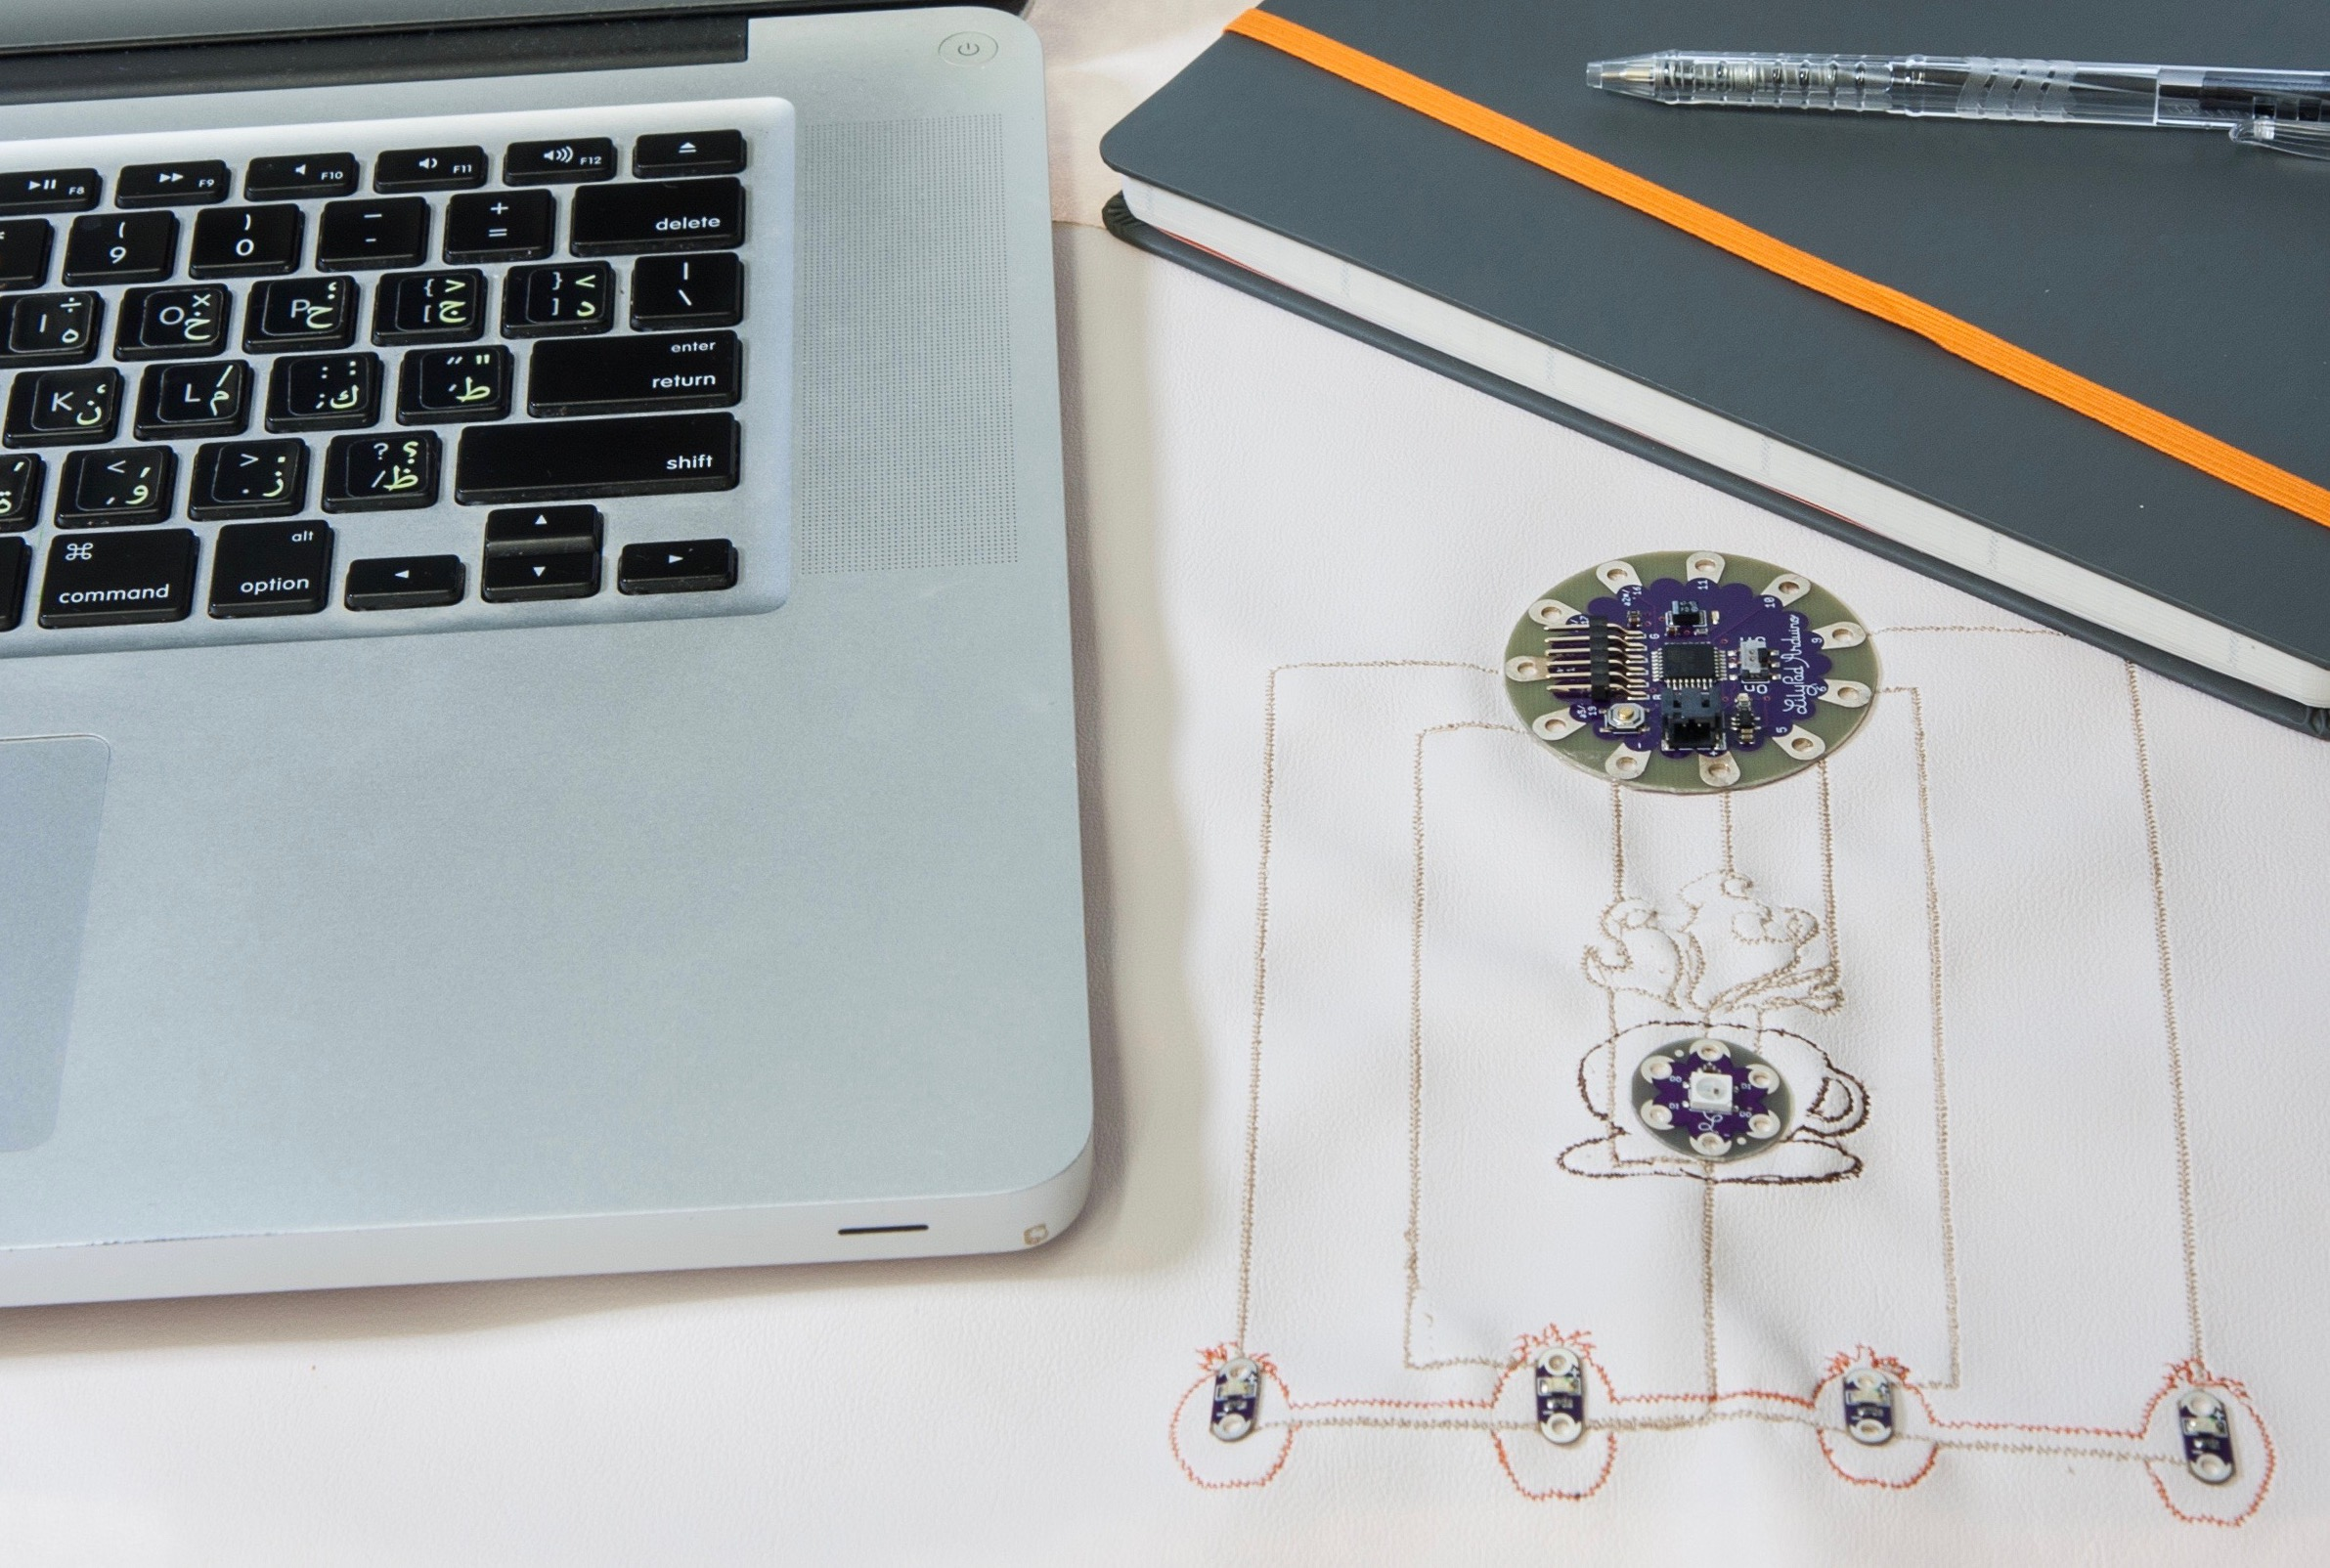
\includegraphics[width=1\columnwidth]{figures/DeskMat}
%   \caption{Example 2: The Interactive Desk Mat. Size 160$\times$130 mm, 9,000 stitches, 3 thread changes, 13 minutes stitch duration.}~\label{fig:DeskMat}
%   \vspace{-1.5em}
% \end{figure}
%The second example is an interactive leather desk mat. 
On leather fabric, the artist sketched an interface for the ``Pomodoro'' time management technique. She used a ruler for sketching, and  4 LEDs, a pixel board, and a controller. She powered the controller from her computer. She programmed a timer to light up an LED every 25 mins to indicate the start of a work interval. Between work intervals, the pixel board blinked to announce a 5 min break. Once all 4 LEDs were lit, the pixel board blinked to announce a longer break.
%Technical lines seemed appropriate for the context of this application. 
She drew traces between the pixel board and controller in the form of steam coming out of the cup (1st integration strategy). 


\subsection{One-Hour Nap Pillow}
% \begin{figure} [h!]
% \centering
%   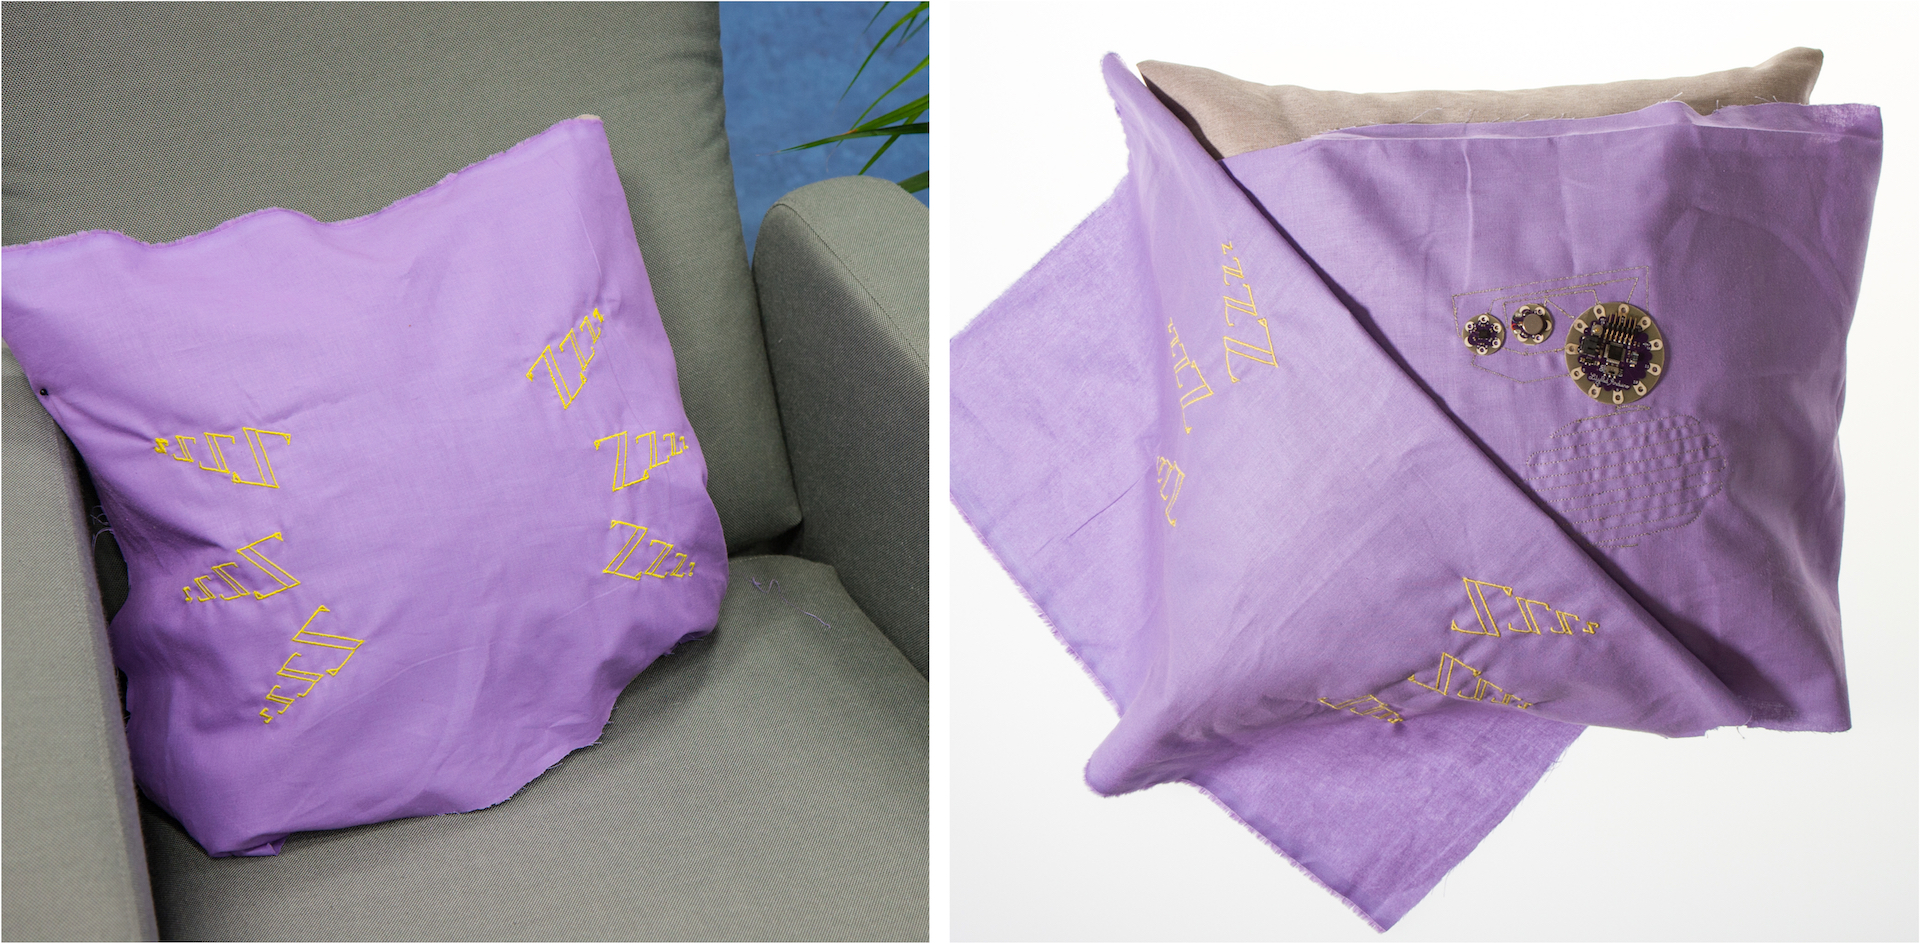
\includegraphics[width=1\columnwidth]{figures/Pillow}
%   \caption{Example 3: The One-Hour Nap Pillow. 16,000 stitches, 2 thread changes, 23 minutes stitch duration}~\label{fig:Pillow}
%   \vspace{-1.5em}
% \end{figure}
The pillow was stitched using our 5th integration strategy---the artwork and circuit were sketched and stitched on separate pieces of fabric and layered afterwards. It contains a touch sensor that detects when a person first puts his head on the pillow, and awakens him using vibration patterns after one hour of continuous contact. The user shakes the pillow to snooze it. An accelerometer signals a 5- or 10-minute snooze based on shaking intensity. On the top fabric, the artist sketched the artwork on one side and used the embroidery machine's touch display to duplicate, mirror, and translate it to the other side. 


\subsection{User Feedback}
The artist was very positive about her experience with our system. She was particularly inspired by the range of circuit integration strategies. We summarize her feedback on the design workflow, sketching on fabric, and design processes. 


\textit{Design Workflow:} The artist found the workflow particularly efficient for creating e-textiles of substantial artwork and simple circuits. She noted that hand-sketching complex circuits can be challenging and error-prone. For example, drawing and correcting the traces in the Wearable Mandala consumed 40\% of the project time. For an 8$\times$8 touchpad sensor, she employed our 5th integration strategy to gain more space to route the sensor traces to a Component Sticker, without affecting her design. She found that using colored pens and stickers for art and circuitry communicate a lower entry threshold. %One limitation is detecting colors on dark colored fabrics. 
After a few trials, she learned how to use the system's feedback to detect and fix digitization pitfalls. Afterwords, she reported that the outcomes of the system better matched her expectations.


%4 hours on the Wearable Mandala: 30 minutes stitching, 10 minutes attaching the electronics using Z-tape, and the remaining time was split between sketching and routing the circuit. 




\textit{Sketching on Fabric:} She reported that a main benefit of sketching on fabric is evaluating designs quickly and in context. While sketching the Wearable Mandala, she wore the t-shirt several times to assess how the design looked, or if it constrained her when moving. Sometimes she made changes to her original layout, e.g., strategically repositioning Component Stickers to convey an idea. Another benefit was understanding the material, e.g., leather inspired straight lines and right angles, while cotton afforded curved and flowing lines. She also noted that textured fabrics, such as denim, caused drawing irregularities, while towel fabric and fur did not afford sketching on them. 


%However, the artist found that our design workflow was not suitable for all fabrics. For example, she reported that drawing continuous lines on stretchable fabrics, which have more than 2\% Elastane, was very challenging. Textured fabrics, such as upholstery fabric, required her to sketch over a single line several times to seal all the gaps in the rough surface. 



\paragraph{Emerging Design Processes}
\textit{Scribble on paper, commit on fabric}. The artist always doodled her initial art and circuit on paper. Fabric was not perceived as a medium for scribbling. Even with undo capabilities, she was hesitant to ``waste a good piece of fabric''. Once her sketch was developed, she transferred it to fabric with adaptations.

\textit{Sketch to fit a circuit:} She sketched the artwork and circuit separately. She then selected an integration strategy based on the complexity of the circuit and the part of the design she wanted to showcase. Next, she gradually transferred the Circuitry Stickers from the circuit to the artwork, drawing the necessary connections and adapting her art, sometimes erasing art lines and replacing them with traces (1st strategy) or routing traces close to art outlines (2nd strategy).

 %In one of her projects, the artist printed a design inspiration she found online and used it to sketch her circuit. She placed Circuitry Stickers on the printed paper and drew traces following design contours. Once she was satisfied with the circuit, she started to sketch her version of the design on fabric with the adaptations. She reported that this technique allowed her to sketch an artwork that fits a circuit instead of fitting a circuit into a design.

\textit{Use stickers to frame the design:} She transferred her sketches from paper to fabric starting with the Circuitry Stickers. This helped her determine the location and scale of the design and evaluate its layout in context before sketching on fabric. 


\section{Limitations and Future work}
Our current digitization algorithm expects pen colors to be distinguishable on the base fabric, and fabrics to have uniform colors and smooth textures. Pens that can release uniform color independent of the applied pressure and fabric background, such as gel-based pens and puffy fabric paint, can neutralize most of the algorithm's pitfalls. But they are harder to undo and their texture may impede stitching over them. Alternatively, augmenting fabric pens to behave like digital pens would allow us to create parallel digital sketches without the previous constraints.
%and the benefits of physical sketching.



%This approach may also benefit the issue of drawing irregularities caused by the fabric texture. Consequently, the embroidery software will not apply a smoothing algorithm which generate lines of varying widths.

%Finally, the system supports two types of stitches---one for filling and one for lines and outlines. Tool proxies with design constraints \cite{mueller2012interactive} could be used to define other stitch types.

Automatic conversion of sketches of many objects often leads to complex tool paths and jump stitches. Trimming jump stitches can be time consuming, and in the case of traces, lead to thread fraying and accidental connections.  We suggest to enable our digitization pipeline to algorithmically reorder individual objects in the embroidery stack to influence the tool path and reduce jumps in the embroidery software.




%As Sketch\&Stitch automates the conversion of freehand sketches to embroidery patterns, jump stitches are very frequent and require trimming to avoid short circuits. High-end embroidery machines offer automatic trimming with a penalty of increased embroidery time. 

Our system does not offer autorouting and rule checks (ERC/DRC) for fabric circuits. It expects users to have a basic understanding of electronics.  %known from PCB layout tools. 
%On one hand, our workflow encourages artistic circuit designs which PCB layout software, such as Eagle, do not support. On another hand, we aim to minimize user interaction with computer screens during the creative tasks. 
In future work, we'd like to examine (a) how to autoroute circuit traces based on the outlines of the artwork, inspired by \cite{savage2014series}, and (b) alternative media, such as augmented reality displays, for real-time feedback.

Finally, we want to perform studies to inspect user requirements and extend our workflow with advanced features, such as stitch selection and manipulation. We aim to conduct a systematic evaluation of our touchpad sensor, and investigate how to stitch a Faraday cage to improve its accuracy. %and a Derivative Integration Algorithm %\footnote{http://www.ti.com/lit/an/snoa939/snoa939.pdf} 


%While users can test their circuit early and frequently in the design process, we believe that embroidery should offer an opportunity for circuit design and validation. 

%Eichinger et al.\ \cite{eichinger2007using} presented early work on using PCB layout software (Eagle) to create embroidered fabric circuits. 

%However, they targeted people who are familiar with PCB layout software.

%One way to improve the accuracy of a capacitive touch sensor is to maintain a constant base capacitance, used as a reference for each measurement. Base capacitance is affected by environmental effects such as temperature and humidity. Texas Instruments for PCB-based capacitive touch sensing \footnote{www.ti.com/lit/an/slaa363a/slaa363a.pdf} recommends two methods for handling this: (1) shielding the sensor with a bottom layer 50\%--75\% hatched ground pour to isolate it from potential interference, e.g., from contact with the skin; and (2) constantly monitoring and tracking variation in base capacitance using, e.g., Derivative Integration Algorithm \footnote{http://www.ti.com/lit/an/snoa939/snoa939.pdf}, for correct comparison to touch events.




%Our capture system cannot distinguish between overlapping lines in a single connection and between two connection.

%The camera capture setup should be well lit to avoid noise from shadows and inconsistent light. 

%In this paper we mainly focused on LilyPad electronics kit. Sketch\&Stitch ca support any off-the-shelf electronics, including DIP and SMD packages, as long as they have a 2.5 mm pitch between leads.
%%trade off between reliable contact surface and smaller contact points.

%The next step for conductive embroidery is to examine using the conductive bobbin thread together with conductive top thread to create multi-layer electrical devices.  

%Ultimately an embroidery machine can be adapted to work like a pick and place machine---placing and stitching electronic components on fabric based on design file. 


\section{Conclusion}
This paper introduced Sketch\&Stitch, an interactive system for creating e-textiles. It enables a new design workflow that combines physical sketching with an embroidery machine, offering users the benefits of direct making and the power of digital tools. %The system is targeted at artists, designers, and makers especially during the early stages of e-textile design. 
It implements a digitization algorithm for converting a sketch to an embroidery. We described novel stitch patterns for attaching electronics, shielding wire crossings, and integrating sensors (pushbuttons, sliders, touchpads) directly on fabric. An empirical evaluation of the technical stitches was presented. Finally, we demonstrated the potential and advantages of our workflow.


%Particular advantages of embroidery machines for e-textile fabrication are that (a) they produce very accurate and consistent stitches over a relatively large surface, (b) their speed, (c) embroidery patterns of circuit elements such as sensors, passive components, antennas, etc., can be pre-programmed, modified, shared, and reused, always providing consistent results, (d) they can be programmed to automatically shield circuit traces, (e) embroidery is an additive manufacturing process that can be use on tailored and finished textiles, 
%reduces the waist created from e-textile fabrication, and finally (f) they are accessible to end users.


%more agency and control over the final outcome \cite{}
% BALANCE COLUMNS
\balance{}

% REFERENCES FORMAT
% References must be the same font size as other body text.
\bibliographystyle{SIGCHI-Reference-Format}
\bibliography{main}

\end{document}
%%% Local Variables:
%%% mode: latex
%%% TeX-master: t
%%% End:
